\chapter{Partidos Políticos, Emendas Parlamentares e Prefeitos: conexão eleitoral \emph{vs} conexão partidária}
\label{cap:emendas}

A literatura brasileira sobre o Congresso Nacional nas últimas décadas demonstrou que os partidos políticos são mais disciplinados e capazes de estruturar o processo legislativo do que se imaginava a partir da derivação direta dos efeitos das regras eleitorais sobre a atuação parlamentar. A despeito da adoção de eleições proporcionais com lista aberta no país, que criaria incentivos para o cultivo do voto pessoal e para a atuação individual e particularista no Legislativo, os partidos políticos na Câmara dos Deputados são bastante disciplinados, previsíveis e orientam as decisões coletivas dos parlamentares (alguns dos principais trabalhos são \citealp*{AmorimNeto2001, AmorimNeto2003, Figueiredo1999a, Figueiredo2000, Figueiredo2002, Figueiredo2008, Limongi2005, Santos1997, Santos1999, Santos2002}).

Por outro lado, diversas pesquisas produziram evidências de que pelo menos parte dos legisladores brasileiros procuram ao longo de seus mandatos obter benefícios particularistas, que garantam sua popularidade frente ao eleitorado e sua sobrevivência política, trocando, inclusive, de partidos quando necessário \citep{Samuels1997, Ames2011, Mainwaring1999, Pereira2001, Pereira2007, Desposato2006}. Há diversas estratégias possíveis para os parlamentares em mandato e concentrar esforços para conseguir levar às suas bases eleitorais benefícios concentrados é uma das opções \citep{Leoni2003, Lemos2011, Desposato } e parlamantares chegam a trocar de partido par

Segundo versões desta vertente, os incentivos ao individualismo parlamentar estariam presentes, mas não se manifestariam no parlamento em virtude das regras internas da Congresso Nacional, que centralizam recursos nas lideranças partidárias, e das diversas prerrogrativas do Executivo nos processos legislativo e orçamentário \citep{Pereira2002, Pereira2003}. As lideranças partidárias seriam as responsáveis pela resolução dos problemas internos de ação coletiva, mas os efeitos dispersivos do sistema eleitoral não estariam eliminados. Assim, a \emph{conexão eleitoral} continuaria existindo, apenas seus efeitos não seriam sentidos nas disputas políticas no interior do Legislativo.

Um dos principais momentos nos quais os parlamentares manifestariam sua preferência em obter benefícios particularistas seria na alocação de recursos orçamentários via emendas parlamentares. Não é por acaso que as emendas parlamentares receberam grande atenção na literatura e no debate político. Na perspectiva distributivista, as emendas individuais ao orçamento forneceriam os recursos fundamentais para a sobrevivência política dos parlamentares, que trocariam localmente benefícios ao eleitores por votos. Assim, em vez de introduzir no orçamento a proposição de bens coletivos, os parlamentares apresentariam emendas que beneficiariam apenas o seu próprio eleitorado, ou \emph{``pork barrel''}, no jargão da ciência política.

De fato, quando questionados sobre a importância das emendas parlamentares em sua carreira política e no seu desempenho eleitoral, os deputados federais tendem a confirmar as expectativas da literatura distributivista. Mais adiante vamos observar alguns dados da Pesquisa Legislativa Brasileira (PLB), survey organizado por Power e Zucco para medir as percepções dos parlamentares no Congresso Nacional sobre diversos temas. Os dados do survey reasseguram que os deputados federais utilizam estrategicamente -- ou, pelo menos, dizem que utilizam -- as emendas parlamentares ao longo do mandato na expectativa de obter votos no futuro nas localidades beneficiadas.

A eficácia dessa estratégia de sobrevivência política por parte dos parlamentares no Congresso Nacional, porém, raramente é questionada (ver \citealp{Mesquita2008}) e os mecanismos da qual dependem nem sempre são examinados.  Em primeiro lugar, os parlamentares precisam ser capazes de introduzir o recurso no orçamento e, posteriormente, conseguir que a emenda seja executada pelo Governo Federal. Em segundo, depende que o beneficiário direto da emenda -- que normalmente é um governo estadual, uma prefeitura ou uma entidade sem fins lucrativos -- transforme o recurso em política pública ou serviço disponível para o cidadão. Também depende do parlamentar ser capaz de reclamar crédito perante os eleitores beneficiados do que foi realizado a partir de sua intermediação no governo federal. Finalmente, para que a \emph{conexão} seja completa, os eleitores precisam recompensar a atuação do parlamentar nas urnas ao final do mandato. Portanto, há vários riscos e incertezas nesta estratégia e convém examiná-los.

O primeiro deles, mais direto, é o Executivo não executar a emenda inserida pelo parlamentar no orçamento. No registro distributivista, as emendas seriam a moeda de troca utilizada pelo Executivo para garantir a aprovação legislativa de sua agenda e este é um dos centros do debate dos estudos legislativos no Brasil. Parlamentares situacionistas teriam maior sucesso do que oposicionistas e, portanto, menor risco ao investir na estratégia de conversão de emendas em votos. \citet{Figueiredo2008} apontam, porém, que mesmo parlamentares de oposição ao Governo Federal conseguem obter algum grau de sucesso na execução de suas emendas individuais e que não há relação causal entre liberação de emendas e apoio legislativo.

Para este capítulo não importa se os parlamentares têm emendas liberadas em função de um processo de barganha com o Governo Federal por apoio no Legislativo ou porque suas preferências são congruentes com as do Executivo. Não há razão, pois, para aprofundar tal debate. Interessa apenas saber que os parlamentares usam de suas prerrogativas para emendar o orçamento com fins eleitorais e, ao mesmo tempo, que têm pelo menos parte de suas emendas executadas.

A maior incerteza para o parlamentar, dessa forma, reside na conversão do benefício obtido aos eleitores em voto. Ainda que o anedotário político esteja repleto de histórias sobre a troca direta de benefícios e votos entre eleitores e representantes eleitos, as evidências empíricas são escassas. Em geral, se assume que os parlamentares são capazes de reclamar crédito por qualquer benefício obtido para um determinada localidade e a simples observação do envio de recursos é tratada como fato que corrobora a narrativa da \emph{conexão eleitoral}. Entretanto, os recursos de emendas parlamentares que podem beneficiar uma localidade têm, em geral, duas formas: a execução de políticas federais na localidade, ou, mais provavelmente, a transferência de recursos mediante convênios, seja para governos estaduais, prefeituras ou para Entidades Sem Fins Lucrativos. Converter uma transferência de recursos para uma organização em um dada localidade em votos não é uma tarefa simples e direta. \citet{Samuels2008} argumenta que o objetivo dos parlamentares sequer é obter votos com a prática de \emph{pork barrel}, mas sim mais recursos de campanha.

Por fim, há também o risco de que os intermediários necessários para que os recursos das emendas executadas não atribuam o crédito ao parlamentar. Veremos adiante que a maior parte dos recursos de emendas que podem ser geograficamente circunscritos beneficiam os governos estaduais ou municipais. E se o governador, prefeito ou dirigente de entidades que recebem os recursos decidirem disputar com o parlamentar a autoria pelo benefício obtido para a localidade? Em particular, e caminhando para o problema deste capítulo, o que ocorre quando deputados federais e senadores têm suas bases eleitorais localizadas primordialmente em estados/municípios governados por partidos aos quais se opõe?

Para que a estratégia de concessão de benefícios particularistas a uma localidade com objetivos eleitorais tenha eficácia, portanto, pelo menos uma condição deve ser satisfeita: as lideranças da organização beneficiária da emenda devem estar dispostas a colaborar com o parlamentar. O argumento central do capítulo, pois, é que deputados federais priorizarão a elaboração e aprovação de emendas que beneficiem atores políticos locais ligados a seu partido -- e não necessariamente um conjunto difuso de beneficiários cuja única propriedade é votar em determinada localidade. Verificar empiricamente se este argumento é verdadeiro é o objetivo da pesquisa apresentada no capítulo. Espera-se que quando deputados federais decidam quais localidades beneficiarão em suas emendas, escolham prioritariamente prefeituras governadas pelo próprio partido e não necessariamente municípios nos quais tem uma boa retrospectiva eleitoral. Assim, mesmo quando os parlamentares atuam de forma particularista, buscando benefícios para o eleitorado de suas bases, o fazem por meio dos canais partidários. Visto sob outra ótica, o objetivo é verificar se o fato do partido governar um município afeta as preferências alocativas dos deputados federais de sua bancadas.

Como se apontou no capítulo anterior, prefeitos são cabos eleitorais privilegiados e capazes de mobilizar votos para as candidaturas do partido a deputado federal e deputado estadual, ainda que a existência desta capacidade esteja condicionada ao contexto eleitoral local, período e às características dos municípios. O impacto de eleger o prefeito no desempenho eleitoral do partido dois anos depois aponta para a existência de algum grau de coordenação entre prefeitos e candidatos a eleições proporcionais dentro dos partidos políticos. Esta relação de apoio é uma via de mão dupla: em troca do suporte eleitoral que são capazes de oferecer, prefeitos demandam de seus pares na Câmara Federal apoio financeiro aos municípios.

O que se espera observar, portanto, é que deputados federais priorizem o envio de emendas parlamentares a municípios governados pelo próprio partido. Argumenta-se que, em vez de focalizar eleitores, os deputados federais preferem concentrar esforços na obtenção de recursos para os prefeitos aliados, cujo apoio afeta diretamente as chances do parlamentar se reeleger. Desta maneira, o deputado consegue dois objetivos: garantir que não haverá algum ator local que dispute a autoria do serviço ou política pública produzida com os recursos da emenda; e garantir que, mesmo se os eleitores não forem diretamente afetados pelo benefício produzido com a emenda, poderá contar ao menos com o apoio do prefeito nas eleições seguintes.

Estendendo o argumento, se prefeitos contribuem para a produção de campanhas vitoriosas a deputados federais, talvez os parlamentares estejam menos preocupados com os efeitos diretos das emendas na intenção de voto dos munícipes e mais interessados no fortalecimento do vínculo com prefeitos. Neste caso, os reais demandantes de \emph{pork} são as lideranças locais, sobretudo prefeitos, e não os eleitores diretos. A enfâse na \emph{conexão eleitoral} e no voto pessoal dada pela literatura distributivista perde parte de seu sentido se, de fato, os partidos políticos são a referência utilizada pelos parlamentares para elaborar emendas individuais ao orçamento inclusive quando o objetivo for beneficiar uma localidade em troca de votos. Em outras palavras, o caminho da \emph{conexão eleitoral} é o próprio partido.

Idealmente, seria possível repetir a pesquisa para deputados estaduais. Entretanto, o processo orçamentário e as possibilidades dos legisladores estaduais apresentarem emendas ao orçamento varia bastante de estado para estado. Além disso, não há dados organizados ou disponíveis para estender a pesquisa para as Assembléias Legislativas. Por outro lado, é possível rapidamente replicar as pesquisas para o Senado Federal, objetivo presente na agenda futura deste trabalho.

A investigação empírica deste capítulo -- se parlamentares privilegiam municípios governados pelo próprio partido ao elaborar emendas -- requer a adoção de estratégias analíticas semelhantes às do capítulo anterior. A expectativa é que parlamentares levem em consideração um conjunto de fatores para a elaboração de uma emenda. Alguns deles estão relacionados tanto à sua performance eleitoral passada quanto ao desempenho eleitoral de seu partido nas eleições municipais que ocorrem no meio de seu mandato. Assim, o desempenho eleitoral do deputado em um município e a probabilidade de elaborar emenda que beneficie tal município estão correlacionados com a probabilidade de seu partido governar o município. Novamente, o desafio metodológico primordial é separar analiticamente a correlação entre desempenho do partido em eleições consecutivas dos efeitos do partido governar o município nas preferências orçamentárias dos parlamentares.

O procedimento de pesquisa, portanto, é semelhante ao do Capítulo~\ref{cap:eleicoes} e utilizo um desenho de regressão descontínua para estimar o impacto do partido vencer as eleições municipais no total de recursos introduzidos no orçamento via emendas elaboradas por parlamentares do partido do prefeito e que beneficiem o governo municipal. Continuando o exemplo fictício utilizado anterioremente, esperamos que a prefeitura de São José do Brasil receba entre 2010 e 2012 \footnote{O período de 2010 a 2012 corresponde ao mandato do prefeito excluído o primeiro ano, 2009. Como se explicará adiante, no momento da elaboração do Orçamento Federal de 2009 há incertezas quanto a quais partidos governarão quais municípios.} relativamente mais recursos dos parlamentares do PMDB, partido vencedor em 2008, do que os municípios em que o PMDB perdeu as eleições para prefeito no mesmo ano.

Os trabalhos sobre a etapa legislativa do orçamento normalmente enfatizam ou a capacidade dos partidos políticos de disciplinar as decisões dos parlamentares, ou a importância das emendas eleitorais para as carreiras dos deputados federais, dependendo da perspectiva teórica e dos propósitos analíticos. Esta pesquisa não coincide com nenhum dos dois tipos de trabalho sobre emendas parlamentares e comportamento legislativo. Assume-se que os parlamentares utilizam suas (restritas) prerrogativas orçamentárias para obter benefícios eleitorais futuros. Há evidências empíricas para acreditar que tal pressuposto seja verdadeiro, como se aponta abaixo. Entretanto, o objetivo é investigar se, mesmo quando supostamente atuam de maneira particularista e perseguem objetivos individuais, não o fazem à revelia do partido, mas sim pelo partido.

O capítulo tem a seguinte estrutura. Na próxima seção, discuto rapidamente alguns aspectos cruciais do processo orçamentário brasileiro no Governo Federal de maneira a situar o problema de pesquisa. A seguir, descrevo os procedimentos de pesquisa e apresento os dados utilizados. Uma vez que o método é o mesmo utilizado no capítulo anterior (desenho de regressão descontínua), abrevio a demonstração das propriedades do RDD e da estratégia de identificação. Entrentanto, examino empiricamente se o uso de RDD é válido para a investigação das hipóteses deste capítulo de maneira breve. Por fim, apresento e discuto os resultados.

\section{Processo Orçamentário no Brasil e Emendas Parlamentares}

O processo orçamentário no Brasil pode ser resumidamente dividido em três etapas. Toda a iniciativa da Legislação Orçamentária é de responsabilidade do Poder Executivo. A primeira etapa constitui, portanto, o envio anual ao Congresso do Projeto de Lei Orçamentária Anual (PLOA) e da proposta Lei de Diretrizes Orçamentárias (LDO) a cada quatro anos e, sempre no primeiro ano do mandato presidencial, de uma proposta de Plano Plurianual (PPA).

A atuação formal do Congresso Nacional está restrita à segunda etapa do processo orçamentário e limitada pelas propostas de legislação formuladas no Executivo. Os diversos atores no Congresso Nacional -- deputados federais, senadores, bancadas e comissões -- podem emendar a proposta recebida do Executivo desde que as emendas não cancelem despesas com custeio (que representa a maior parte do orçamento), não produzam despesas que não tenham indicação da fonte de recursos e, por fim, se adequadem às diretrizes da LDO e do PPA. Em síntese, os parlamentares estão limitados à realocação dos recursos destinados ao investimento e o Congresso Nacional apenas autoriza o orçamento. É nas emendas que os parlamentares apresentam ao orçamento, portanto, que podemos observar suas preferências alocativas.

Por fim, a terceira etapa do processo é a execução do orçamento pelo Poder Executivo. Como o orçamento brasileiro não é mandatório, ou seja, não produz obrigatoriedade de execução do que foi aprovado pelo Congresso Nacional, o Executivo tem grande margem de discricionaridade para determinar quais gastos serão realizados. Adicionalmente, a própria legislação orçamentária permite ao Executivo a realocação de recursos entre rubricas, ainda que com severos limites. 

Portanto, a iniciativa exclusiva do Executivo na legislação orçamentária e sua capacidade de remanejar recursos e contingenciar gastos circunscreve consideravelmente a atuação formal do Congresso Nacional. As emendas apresentadas por parlamentares sofrem restrições quanto à sua capacidade de alterar as preferências do Executivo e não se traduzem necessariamente em recursos dispendidos. Os recursos introduzidos no Orçamento Federal mediante emenda dependem do resultado final da LOA aprovada no Congresso Nacional e da ação discricionária do Poder Executivo.

As emendas individuais dos parlamentares, foco deste capítulo, não são os únicos instrumentos disponíveis aos deputados federais. Os parlamentares podem apresentar emendas coletivas (pelas bancadas regionais, bancadas estaduais e comissões). Além disso, o relator geral do orçamento e os relatores parciais também podem emendar o orçamento. %As emendas ao orçamento apresentadas pelo Congresso Nacional de 2002 a 2012 foram responsáveis por apenas XX\% das despesas totais com investimento no Orçamento da União e XX\% de todas as despesas.
Se não se pode assumir, portanto, que os recursos de emendas parlamentares provoquem alterações relevantes para o Poder Executivo (como descrevem \citealp*{Figueiredo2008}) o contrário não é válido. Não apenas os recursos provenientes de emendas parlamentares importam para os membros do Legislativo como também a ação do Executivo interfere diretamente no sucesso dos deputados federais e senadores na realização de suas preferências orçamentárias.

Uma avaliação apressada dos aspectos formais do processo orçamentário levaria à conclusão de que apenas o Poder Executivo, portanto, tem alguma possibilidade de realizar transferências de recursos aos municípios brasileiros. Entretanto, os parlamentares tentam constantemente obter a execução de suas emendas parlamentares durante seu mandato, inclusive os parlamentares da oposição, e têm relativo sucesso.

Uma importante evidência de que as emendas são relevantes para pelo menos um grupo grande de parlamentares no Congresso Nacional é a tentativa de tornar obrigatória a execução de emendas por parte do Executivo. Nos meses em que o texto final desta tese estava sendo elaborado, o Senado votou em plenário e aprovou uma Proposta de Emenda Constitucional (PEC) que tornaria mandatória a execução pelo Poder Executivo das despesas inseridas no Orçamento Federal por emendas parlamentares. Apesar da Presidência ser contra a alteração das regras orçamentárias, a aprovação da PEC no Senado contou inclusive com os votos de membros da base do governo. A Câmara dos Deputado já havia votado e aprovado uma versão modificada anterioremente do projeto. Mais ainda: nos últimos dias de 2013 houve acordo entre a Presidência e o Congresso Nacional para que constasse na LDO de 2014 a obrigatoriedade da execução das emendas parlamentares.

Há interesse por parte de deputados e senadores, portanto, em garantir a execução de suas emendas e alterar as regras do processo orçamentário. Esta é uma posição que não parece depender de partido político ou de posicionamento em relação ao Governo Federal. Vamos examinar na próxima seção como os próprios parlamentares atribuem importância às emendas aprovadas no orçamento.

\subsection{Emendas ao orçamento, lideranças locais e carreira política: a percepção dos próprios parlamentares}

O objetivo deste capítulo é investigar se deputados federais privilegiam municípios governados por membros de seu próprio partido ao introduzir emendas no orçamento. O argumento central é que as emendas individuais importam para o futuro eleitoral dos deputados federais, mas que o beneficiário fundamental das emendas são as liderenças locais vínculadas ao partido do parlamentar e não os eleitores.

O pressuposto subjacente a este problema de pesquisa é que as emendas individuais ao orçamento importam para os deputados federais. Importar, neste caso, deve ser lido como ``ter relevância'' e não necessariamente como ``ter efeito''. Pode ser que a estratégia de introduzir emendas no orçamento com finalidades eleitorais não afete as chances do parlamentar se reeleger \citep{Mesquita2008}. Contudo, interessa exclusivamente se os parlamentares acreditam que suas emendas individuais têm impacto em suas carreiras políticas e se orientam no Congresso por esta crença.

Para investigar a validade deste pressuposto, utilizo dados da Pesquisa Legislativa Brasileira, um \emph{survey} aplicado por Timothy Power e Cesar Zucco nas últimas seis legislaturas do Congresso Nacional. Em particular, o questionário da última edição do \emph{survey}, realizada em 2009, traz perguntas que são interessantes para este capítulo.

A primeira delas -- e mais relevante -- é bastante simples: ``Na sua opinião, que importância tem aprovar e obter a execução de emendas ao orçamento para o futuro eleitoral de um congressista: nenhuma, alguma, muita?''. Dos 135 parlamentares que responderam a esta pergunta, quase dois terços (62,2\%) afirmou que as emendas ao orçamento têm muita importância para o futuro eleitoral de um parlamentar. Mais de um terço (35,5\%) afirmou que as emendas têm alguma relevância. Apenas 2,2\% dos parlamentares acreditam que emendas ao orçamento não estão relacionadas ao futuro eleitoral de um deputado federal ou senador.

Os parlamentares também responderam na edição de 2009 do \emph{survey} sobre a importância que o encaminhamento de demandas de prefeitos ou lideranças locais têm sobre seu futuro eleitoral\footnote{A pergunta no \emph{survey} é: ``Na sua opinião, que importância tem o encaminhamento das demandas dos prefeitos ou lideranças locais para o futuro eleitoral de um congressista: nenhuma, alguma, muita?''}. Mais da metade (53,7\%) disse que o atendimento de tais demandas é muito importante e 44\% atribui alguma importância. Só três parlamentares dos que responderam à pesquisa não acreditam que atender a líderes locais impacte na carreira de um parlamentar, dois dos quais também não dão importância a emendas ao orçamento.

Por fim, a comparação entre a importância do atendimento a demandas de prefeitos e liderenças locais com o atendimento a pedidos de eleitores, também perguntado no \emph{survey}\footnote{A pergunta no \emph{survey} é: ``Na sua opinião, que importância tem o atendimento aos pedidos de eleitores para o futuro eleitoral de um congressista: nenhuma, alguma, muita?''}, aponta na direção da intuição apresentada na introdução da tese: de que os demandantes de \emph{pork} são os governantes locais e não os cidadãos do município. Se 53,7\% consideram muito importante atender a prefeitos e líderes locais, apenas 31\% considera muito importante atender diretamente os eleitores. A grande maioria (quase 61,5\%) considera que atender a pedidos de eleitores têm alguma importância e 7,5\% não dão importância alguma. Demandas de eleitores são importantes, mas menos do que as demandas de outros atores políticos locais na visão dos próprios deputados federais.

Os resultados para a legislatura de 2007-2010 são bastante claros: atender a demanda de prefeitos e líderes locais e introduzir emendas ao orçamento, na percepção dos parlamentares, são ações que afetam seu desempenho eleitoral. Os dados da Pesquisa Legislativa Brasileira apontam, portanto, que parece seguro assumir que os parlamentares atribuem relevância às emendas parlamentares, mesmo em um contexto em que as prerrogativas do Congresso no processo orçamentário sejam bastante limitadas. Os recursos destinados à execução das emendas parlamentares ao orçamento, sobretudo às emendas individuais, não representam uma parcela relevante da despesa do Governo Federal com investimento, mas são recursos cruciais para os parlamentares e no atendimento das demandas de políticos e lideranças locais.

Na próxima seção, apresento algumas informações sobre as emendas individuais ao orçamento e transferências aos municípios. Em particular, é fundamental refletir sobre como medir a preferência alocativa dos parlamentares eleitos.

\subsection{Transferências intergovernamentais e emendas parlamentares: o quê medir?}

A distribuição de recursos entre os diferentes níveis de governo em países federativos é um dos principais aspectos que moldam as relações intergovernamentais. Um dos focos da literatura de política econômica são as consequências políticas das transferências de recursos dos governos centrais para os governos locais. De um lado, as transferência são instrumentos disponíveis aos formuladores de políticas públicas para a redistribuição de recursos entre os governos locais e potencialmente para a redução de desigualdades. De outro, a alocação discrionária de recursos a serem transferidos para outros governos é um instrumento estratégico na mão dos partidos políticos e que pode ter consequências eleitorais relevantes. Diversos trabalhos demonstraram que os governos centrais privilegiam a transferência de recursos a localidades controladas por membros do seu partido ou nas quais está presente uma parcela do eleitorado, seja de \textit{core voters} ou \textit{swing voters}, relevante para suas estratégias eleitorais.

No Brasil, a maior parte das transferências do governo federal a estados e municípios é determinada por regras fixas. Entretanto, um volume significativo de recursos transferidos depende da ação discricionária de atores federais. Entre 2002 e 2012, as transferências voluntárias representaram cerca de 18\% do total repassado aos estados e aos municípios\footnote{fonte: elaboração própria a partir de IPEADATA}. Os recursos no Orçamento Federal sobre os quais é possível decidir mais livremente a alocação são diversos e dentre eles se incluem aqueles inseridos durante o processo orçamentário por meio de emendas parlamentares.

No período de 2002 a 2012 o Congresso Nacional apresentou aproximadamente 110 mil emendas ao PLOA. Quase 90 mil foram emendas individuais, enquanto as demais foram elaboradas pelos relatores, comissões ou bancadas regionais e estaduais de ambas Casas Legislativas. Somadas, as emendas individuais correspondem a XX\% do total de despesas introduzidas por emendas parlamentares no texto final da Lei Orçamentária Anual (LOA) enviado para o Executivo. As emendas individuais representam uma parcela expressiva da atividade dos membros do Legislativo Federal e o momento de sua elaboração é uma das poucas situações ao longo do mandato em que o parlamentar pode transformar suas preferências em ações do Estado.

Dado que o objetivo deste capítulo é estimar o impacto do partido governar o município na decisão dos parlamentares do partido de alocarem recursos federais para este município, é preciso capturar o momento em que as preferências dos membros do partido no Legislativo são reveladas e podem ser medidas. Assim, diferentemente de outros trabalhos sobre transferências de recursos federais para municípios, interessa observar apenas as emendas individuais, cuja autoria é facilmente atribuída a um parlamentar e, consequentemente, corretamente atribuída a um partido.

Somente com as emendas individuais e que produzam transferências de recursos para um município, ou para uma organização localizada no município, servem para análise. As transferências voluntárias totais aos municípios não refletem apenas a decisão dos partidos no Congresso, mas também do Poder Executivo. As emendas de bancadas ou comissões expressam preferências de um conjunto de parlamentares que não necessariamente pertencem a um mesmo partido. As emendas dos relatores, por sua vez, não são comparáveis às dos legisladores individuais pelas desigualdades de atribuições dos relatores em relação aos demais membros do Legislativo no processo orçamentário. Uma vez que identificar com precisão o partido político do autor da emenda é crucial para a análise, as transferências voluntárias que não têm origem nas emendas parlamentares, as emendas de bancada, comissões ou de relatores são desconsideradas. 

Em síntese, para medir a preferência geral de um partido na alocação de recursos orçamentários entre municípios, a melhor alternativa é utilizar a soma das emendas individuais de seus parlamentares. Este é o procedimento adotado neste capítulo. Ainda que o volume de recursos provenientes de outros tipos de emendas ou fontes que um município recebe possa depender também de qual partido governa a prefeitura, incluí-los não contribuiria para a presente análise.

A Câmara dos Deputados foi responsável pela confecção de cerca 87\% das emendas individuais apresentadas no Congresso Nacional de 2002 a 2012. Os deputados federais apresentaram aproximadamente 79 mil emendas individuais ao PLOA. Todas as emendas apresentadas descrevem onde o recurso, se aprovado e executado, será gasto: em um município, estado ou mesmo em uma região do país. Ao todo, separando as emendas pelas localidades beneficiadas, apenas, obtém-se aproximadamente 156 mil ``itens''. É bastante comum que deputados apresentem emendas com vários ``itens'' e que destinem recursos para seu próprio estado e para um ou mais municípios dentro do estado ao mesmo tempo, por exemplo. Para manter a simplicidade do texto e da análise, considerarei cada ``item'' uma ``emenda''.

Destas 156 mil emendas individuais apresentadas na Câmara dos Deputados no período de análise, apenas 6,2\% tinha como destino regiões. A grande maioria (57,3\%) tinha como beneficiário algum estado, normalmente o estado pelo qual o próprio parlamentar foi eleito. Pouco mais de um terço, 36,6\% (que corresponde a quase 58 mil emendas), contemplavam municípios. A apresentação de emendas que tenham finalidade o município é, portanto, um componente relevante da atuação dos parlamentares.

Da mesma forma que é preciso concentrar a análise nas emendas individuais para poder atribuir corretamente cada emenda a um partido, serão consideradas no capítulo somente as emendas que tenham como destino os municípios. O envio de recursos de emendas (ou, mais precisamente, itens de emendas) a estados ou regiões não depende de qual partido governa a prefeitura e pode ser descartado da análise. No momento em que houver informação precisa sobre quais partidos participam das coalizões nos estados -- tarefa à qual os membros do projeto de pesquisa no qual esta tese está inserida têm se dedicado -- será possível observar o efeito dos partidos governando os estados na decisão dos membros do partido no Congresso. Na ausência desta informação, o procedimento adequado é produzir a análise exclusivamente a partir das emendas cujos beneficiários são os municípios, denominadas a partir deste momento de ``emendas municipais''.

Tomar o município como beneficiário da emenda parlamentar também não é suficientemente preciso. Ao elaborar a emenda, o parlamentar pode decidir sobre diversos aspectos da despesa que pretende inserir no orçamento além da localização final. Pode optar, por exemplo, pela área de política em que a despesa estará inserida, de qual órgão do governo federal virá o recurso, se envolverá a execução direta de uma política pelo Governo Federal ou a transferência para outra organização executá-la.

Para os objetivos do capítulo, interessa saber quem é o beneficiário da emenda. Além de separar as emendas pelo partido de autoria e a pelo município ao qual o recurso se destina, portanto, separarei as emendas também pelo tipo de beneficiário dentro do município. Quase dois terços das emendas municipais -- 37 mil das 58 mil emendas -- têm como finalidade a transferência de recursos para prefeituras. Estas 37 mil emendas são as que mais interessam à presente análise pois são aquelas que transferem recursos para que os prefeitos executem políticas públicas federais. Se, de fato, deputados federais privilegiam prefeitos aliados, então devemos observar uma frequência maior de emendas dos deputados para prefeituras em que o seu próprio partido venceu do que em prefeituras em que o partido perdeu as eleições para prefeito.

Uma quantidade relevante de recursos introduzidos no Orçamento Federal mediante emendas parlamentares, por outro lado, tem como beneficiário Entidades Sem Fins Lucrativos (ESFL). De 58 mil emendas individuais municipais, pouco menos de 8 mil nos 11 anos incluídos na análise deram a origem a convênios entre o governo federal e ESFLs. Tais emendas também são de grande interesse para a análise. ESFLs podem configurar uma rota alternativa para deputados federais enviarem recursos a apoiadores políticos em municípios governados por prefeitos de outros partidos. Explorarei este tema adiante.

São consideradas na análise, portanto, as emendas enviadas diretamente para as prefeituras e as emendas enviadas diretamente a ESFLs. Há outras maneiras de beneficiar um município com emendas. Por exemplo, políticas executadas pelo Governo Federal nos municípios são um benefício para a prefeitura semelhante à transferência de recursos. Entretanto, é bastante difícil atribuir com precisão o beneficío a um ator político local posicionado contra ou a favor de um partido nestes casos. Dessa forma, aplicação direta de recursos federais no município e outras formas de transferência são ignoradas. A grande maioria das emendas são transferências de recursos a prefeituras ou a ESFL. As transferências totais no município têm variação similar às transferências a prefeituras e sua inclusão na análise não traz novas informações.

É necessário notar que a expectativa em relação às emendas que beneficiam ESFL é oposta à expectativa das emendas que beneficiam diretamente a prefeitura. Por qual razão os parlamentares decidiriam enviar recursos a ESFLs em municípios nos quais têm o prefeito como aliado? Uma resposta possível, adotada como hipótese nesta tese é: as ESFL podem representar um caminho alternativo para a obtenção de apoio eleitoral em municípios governados por opositores. Se interessa a um parlamentar conquistar votos em um município que é governado por um prefeito de outro partido, o apoio de dirigentes de ESFLs pode ser uma alternativa.

Há, porém, outra resposta possível: ESFLs podem representar uma rota para envio de recursos demandados pelo prefeito sujeita a menos controles procedimentais e burocráticos do que a prefeitura. Neste caso, o demandante de recursos continua sendo um prefeito aliado e o que muda em relação a transferências diretas à prefeitura é o meio pelo qual os recursos chegam ao município e a capacidade do governo federal e Tribunais de Contas fiscalizarem a utlização destes recursos.

As duas respostas apontam para direções opostas. Em um caso, esperamos relação negativa entre o partido governar o município e o total de recursos que a bancada do partido na Câmara dos Deputados destinará às ESFLs sediadas no município. No outro caso, esperamos uma relação positiva, posto que o demandante local do recurso pertence ao mesmo partido dos deputados que introduziram a emenda no orçamento. Não é inviável também que ambas as respostas estejam simultaneamente corretas e que as duas motivações para apresentação de emendas que beneficiem ESFLs existam.

Há um último ponto crucial na observação das preferências dos parlamentares e seus partidos no Orçamento Federal por meio das emendas: em que etapa os valores das emendas devem ser medidos? No autógrafo das emendas? No texto da LOA aprovado no Congresso? Na LOA sancionada pela Presidência? Na execução orçamentária? Nos valores efetivamente pagos/transferidos?

Na etapa do processo orçamentário que envolve formalmente o Congresso Nacional, os legisladores podem apresentar livremente suas preferências, desde que respeitados as regras e limites de valores estabelecidos para as emendas. Assim, o valor apresentado nas emendas deve ser mais próximos da preferência real -- sincera e irrestrita -- dos parlamentares do que qualquer outro valor que se possa medir durante a elaboração e execução do orçamento. Entretanto, como o Congresso tem atuação bastante limitada e a prerrogativa de realizar ou não uma despesa é do Poder Executivo, o valor apresentado não é igual ao montante de recursos gasto em benefício do município. Para que haja uso estratégico das emendas, como se argumenta nesta tese, não basta ao parlamentar apresentá-las ao orçamento. É preciso também garantir sua execução.

O segundo problema com a utilização dos valores apresentados -- e não necessariamente realizados -- é que os parlamentares inserem no orçamento emendas considerando estrategicamente aquelas que têm maiores probabilidades de serem executadas. Diversos fatores podem contar a favor disso, tais como suas conexões no órgão do Governo Federal responsável pela execução, sua capacidade de barganhar com a Presidência ou ainda por quem será o beneficiário da emenda. Se há barganha entre Poderes e o Executivo também decide estrategicamente sobre quais emendas serão executadas, o valor apresentado das emendas não revela necessariamente uma preferência sincera, mas sim uma preferência estratégica do parlamentar.

Ambos os aspectos seriam bastante problemáticos se, por exemplo, somente parlamentares de partidos no governo obtivessem algum sucesso na execução de emendas. Em um cenário como este, deputados e senadores de oposição poderiam desistir, por exemplo, de apresentar emendas. Ou apresentariam as emendas como mera justificativa formal aos prefeitos e lideranças locais de que atuam em benefício de determinada localidade. Entretanto, na próxima seção descrevo e apresento os dados utilizados no capítulo e, como se verá, nenhuma dessas conjunturas parecem plausíveis. Parlamentares de todos os partidos apresentam emendas e o total por bancada corresponde ao número de parlamentares de cada partido.

Substituir o valor apresentado originalmente pelos parlamentares nas emendas pelo valor que consta na LOA após a sanção presidencial não altera o problema. Pelo contrário, adiciona o ruído provocado pela interação entre os parlamentares e os relatores e comissões de orçamento no Congresso. Restaria, assim, observar os valores empenhados ou pagos de emendas que foram efetivamente executadas. No entanto, quanto mais longe os valores estiverem do processo de elaboração das emendas, situado no início da fase congressual do processo orçamentário, mais difícil fica argumentar que tais valores refletem as preferências dos parlamentares. Elas são o resultado observado do processo de interação e da eventual disputa entre os Poderes. Ainda que deputados e senadores possam influenciar quais de suas emendas serão aprovadas, nenhuma das duas medidas (valores empenhados ou valores pagos) reflete o que se gostaria medir.

O valor apresentado continua sendo, portanto, a medida mais próxima do que se pretende capturar: a preferência sincera e irrestrita dos parlamentares na alocação de recursos entre municípios. Mesmo que não representem os recursos federais efetivamente dispendidos ou transferidos para os municípios, os valores que constam orginalmente nas emendas seguem sendo a melhor aproximação do que se quer estudar. Se todos os partidos têm  pelo menos parte de suas emendas executadas, então é razoável assumir que os parlamentares e bancadas partidárias em geral esperam que o uso estratégico de emendas tenha alguma eficácia. De qualquer forma, é prudente examinar os efeitos heterogêneos entre governistas e situacionistas, e assim procedo no capítulo.

Antes de descrever os dados utilizados, discuto brevemente como um desenho de regressão descontínua, que já foi detalhado no capítulo anterior, é adequado para a investigação do problema de pesquisa deste capítulo.

\section{Procedimentos de Pesquisa: Regressão Descontínua, eleições para prefeito e emendas individuais ao orçamento}

No Capítulo~\ref{cap:eleicoes}, apresentei como desenhos de regressões descontínuas têm sido adotados com frequência na ciência política para estimar o efeito do partido vencer as eleições majoritárias sobre uma variável potencialmente afetada pela vitória. Eleições majoritárias produzem uma variação quase aleatória no tratamento entre as observações próximas ao ponto de descontinuidade (margem de vitória igual a zero) que, consequentemente, viabilizam a estimação de efeitos causais da vitória eleitoral. Ou, sob outra ótica, permitem estimar os efeitos de um partido específico governar um município sobre um conjunto de variáveis tais como o total de recursos transferidos ao município que resultam da atuação dos parlamentares daquele partido. Neste capítulo, mudaremos a linguagem de ``impacto de vencer as eleições'' para ``impacto do partido governar um município'', tendo em vista que, dada a estratégia metodológica, essas duas formas de interpretar o tratamento são equivalentes. Vamos rapidamente rever a mecânica da regressão descontínua antes de avançar para os dados do capítulo.

\subsection{A mecânica da regressão descontínua: emendas individuais ao orçamento}

Como vimos anteriormente, a votação de um partido $p$ no município $m$ para uma eleição para prefeito no ano $t$ ($V_{p,m,t}$ ou $V_{i}$, sendo $i$ uma combinação de $p$, $m$ e $t$) pode ser descrita em termos de uma função densidade de probabilidade condicional às diversas características do partido no município, representados por $A_{i}$ e assumidos aqui como não observáveis, e por um termo aleatório $\epsilon_{i}$. 

Nos municípios brasileiros com menos de 200 mil eleitores aptos, os candidatos disputam uma eleição majoritária de apenas um turno para a prefeitura e vence as eleições o candidato que obtiver o maior número de votos $V_{i}$. Governará o município o partido ($d_{i}=1$) que tiver maior $V_{i}$ e, portanto, margem de votos positiva em relação ao partido oponente mais bem votado ($\tau_{i}=\Delta>0$) na eleição municipal. Os demais partidos, com margens de votos negativas ($\tau_{i}=-\Delta<0$) em relação ao primeiro, não são eleitos ($d_{i}=0$) e, portanto, fazem parte do grupo de controle, composto pelos partidos que não governam o município. Cada partido tem uma probabilidade diferente de governar ou não o município e esta probabilidade depende de $A_{i}$.

O objetivo é estimar o efeito do tratamento $d_{i}$ em $Y_{i}$, que é uma variável resposta que pode ser descrita da mesma forma que $V_{i}$ e também é função de $A_{i}$. Como $d_{i}$ e $Y_{i}$ são função dos mesmos conjuntos de variáveis, a condição de independência $Y_{i} \perp d_{i}$ não é válida. Entretanto, como vimos no primeiro capítulo, quando o módulo margem de vitória ($\Delta$) tende a zero temos que a probabilidade de um partido vencer a disputa em um município e em uma eleição específica é independente do fatores não observáveis ($A_{i}$) que determinam $\tau_{i}$. Logo: 

\[
\lim_{\Delta \to 0} E[d_{i}|\tau_{i}=-\Delta]=\lim_{\Delta \to 0} E[d_{i}|\tau_{i}=+\Delta]
\]

A consequência do tratamento ser quase aleatório é que podemos estimar o efeito de $d_{i}$ (ou do o partido $p$ governar o município $m$ após a eleição $t$) em $Y_{i}$ da seguinte maneira:

\[\rho =\lim_{\Delta \to 0} E[E[Y_{i}|d_{i}=1]|\tau_{i}=+\Delta] - \lim_{\Delta \to 0} E[E[Y_{i}|d_{i}=0]|\tau_{i}=-\Delta]\]
\[=\lim_{\Delta \to 0} E[Y_{1,i}|\tau_{i}=+\Delta] - \lim_{\Delta \to 0} E[Y_{0,i}|\tau_{i}=-\Delta]\]
\[=\lim_{\Delta \to 0} (E[Y_{1,i}|\tau_{i}=+\Delta] - E[Y_{0,i}|\tau_{i}=-\Delta])\]

Tal como no primeiro capítulo, o efeito causal estimado, $\rho$, será sempre apresentado em função de $\Delta$, posto que a arbitrariedade na escolha da margem de vitória pode levar a resultados fortuitos. Da mesma maneira, em diversos momentos $\rho$ é estimado de três maneiras diferentes: como diferença de médias entre os grupos de tratamento, como descontinuidade em um função linear de $Y_{i}$ por $\Delta$ e como descontinuidade em um função polinomial de terceiro grau de $Y_{i}$ por $\Delta$.

\subsection{Operacionalização da pesquisa, hipótese e dados utilizados}

A unidade de análise na pesquisa deste capítulo é novamente o partido ($p$) em um município ($m$) e em uma eleição ($t$). Quando o partido $p$ vence as eleições $t$ no município $m$ e, portanto, governa o município nos quatro anos seguintes, ele integra o grupo dos tratados ($d_{i}=1$). Se $p$ foi derrotado, ele compõe o grupo de controle ou não tratados ($d_{i}=0$). O objetivo neste capítulo é testar se os parlamentares do partido $p$ destinam mais recursos por meio de emendas individuais ao Orçamento Federal aos municípios governados pelo partido do que aos municípios não governados pelo seu partido, sendo esta a hipótese principal do capítulo.

Integram o conjunto de dados os dois partidos mais bem colocados nas eleições para prefeito em municípios com menos de 200 mil eleitores aptos e que, portanto, não têm possibilidade da disputa ser decidida em dois turnos. $V_{i}$ é medido como o percentual de votos que o partido $p$ teve nas eleições $t$ no município $m$ e $\tau_{i}$ é a diferença entre os dois competidores, sendo positiva para o vencedor e negativa para o perdedor. 

A variável resposta, $Y_{i}$, é a soma dos valores das emendas apresentadas pelos deputados do partido $p$ que beneficiam o município $m$ nos anos seguintes à eleição $t$, exceto o primeiro, e pode ser construída com quatro denominadores diferentes: 1 - o total de eleitores aptos a votar; 2 - o total de receitas orçamentárias do município; 3 - total de emendas apresentadas pelo partido a todos os municípios naquele ano; ou 4 - o total de emendas apresentadas ao município por todos os partidos no mesmo período. Voltemos ao exemplo fictício de São José do Brasil, em que o PMDB foi o partido vitorioso em 2008 e o PSDB terminou a eleição em segundo colocado. Vamos supor que três deputados federais do PMDB apresentaram emendas individuais ao orçamento entre 2010 e 2012 que destinam recursos ao município São José do Brasil. O numerador $Y_{i}$ para o PMDB neste município e em 2008 é a soma das emendas dos três deputados nos anos nos quais o partido governou o município, exceto no primero ano de governo, dividido por algum dos três denominadores acima apontados.

No exemplo do PMDB em 2008 e em São José do Brasil, o primeiro denominador é o número de eleitores aptos nas eleições de 2008 no município. Este denominador poderia ser facilmente substituído pelo total de votos válidos ou pelo total de habitantes sem que o resultado fosse relevantemente alterado, exceto na magnitude dos coeficientes estimados. A escolha por eleitores aptos resulta da interpretação de que o parlamentar apresenta emenda esperando votos do município no futuro, ainda que por intermédio do prefeito, como já debatido, o que torna o número de eleitores apto um divisor adequado para o problema.

O segundo denominador é simplesmente a receita orçamentária municipal em $t$. Com este denominador, é possível calcular a proporção que as transferências de emendas individuais do partido $p$ para o município $m$ representam da receita municipal. A vantagem desses dois primeiros denominadores é que a dimensão do município é controlada, pois quanto maior a população do município, maiores as receitas da prefeitura e o volume de recursos que os parlamentares destinam ao município por meio de emendas individuais.

O terceiro denominador é a soma dos valores de todas as emendas individuais que os parlamentares do PMDB apresentaram entre 2010 e 2012 destinadas a qualquer município (excluídas, portanto, as emendas que beneficiavam regiões ou estados inteiros). Medindo $Y_{i}$ desta maneira, temos uma ideia clara da divisão do orçamento de emendas individuais de cada partido no Congresso entre municípios e podemos observar facilmente a diferença entre localidades nas quais o partido governa e nas quais perdeu as últimas eleições para prefeito.

Por fim, o último denominador é a soma dos valores das emendas individuais de parlamentares de todos os partidos que beneficiavam São José do Brasil entre e 2010 e 2012. Ao optar por este denominador, sabemos se o partido vitorioso aumenta sua participação no envio de recursos ao município. Esta variável, porém, traz consigo alguns problemas abaixo explorados. Como muitos municípios pequenos não recebem nenhum recurso da maioria dos partidos ou recursos de um só partido, a variável tem muitos valores extremos (zero e 100\%).

Note-se que, como a LOA deve ser aprovada até o final de agosto de cada ano e as eleições ocorrem em outubro, em $t$ os parlamentares não sabem qual será o partido do prefeito no ano seguinte. Assim, é necessário excluir as emendas inseridas no orçamento e que beneficiem o município no primeiro ano do mandato de qualquer prefeito. No exemplo hipotético, o ano de 2009 está excluído e $Y_{i}$ é a soma dos valores de emendas individuais do partido $p$ que beneficiem o município $m$ nos três últimos anos do mandato do prefeito, ou seja, 2010, 2011 e 2012.

Há diversas formas pelas quais um deputado federal consegue destinar recursos a um município via emenda parlamentar ao orçamento. A primeira delas e mais comum é destinando recursos diretamente à prefeitura ou a uma Entidades Sem Fins Lucrativos (ESFLs) situada no município. Exemplos de ESFLs são hospitais beneficentes e Santas Casas, associações, centros comunitários, entidades sindicais, cooperativas, etc. Além disso, é possível aprovar uma emenda que determine a execução de uma política pública do Governo Federal no Município. Na linguagem do orçamento público brasileiro, há diversas modalidades de aplicação nas quais as emendas individuais podem estar classificadas.

No capítulo, a variável dependente $Y_{i}$ será medida de duas maneiras lenvando em consideração a classificação da emenda por modalidade de aplicação e para as quais estabeleço hipóteses com sinais opostos. A primeira é composta apenas pelas transferências diretas à prefeitura (modalidade de aplicação 40 e 41 e representada por $Y_{i}^{pref}$ ). A vantagem de medir $Y_{i}$ desta maneira reside na atribuição precisa do benefício de uma emenda individual do parlamentar de um partido a um outro ator político cujo partido também é conhecido. A migração de prefeitos e deputados federais certamente provoca ruído na análise, mas é desconsiderada nesta pesquisa. Felizmente, a migração partidária tornaria menos provável a obtenção de resultado positivo e podemos assumir que os efeitos da vitória para prefeito verdadeiros são iguais ou maiores aos que forem estimados no capítulo.

$Y_{i}$ também é medido apenas como transferências a ESFLs (modalidade de aplicação 50 e representada por $Y_{i}^{esfl}$). Quando se tratar de transferências a ESFLs o procedimento é exatamente o mesmo, com a diferença que as emendas individuais têm como beneficiário uma organização localizada no município $m$. É importante lembrar que, quando $Y_{i}$ mede transferências a ESFLs, a hipótese não tem sinal pré-definido: é possível que parlamentares destinem mais recursos para entidades em municípios governados por outros partidos em comparação com municípios governados pelo seu próprio partido ou o contrário. Esta hipótese será discuta adiante com mais cuidado. Por enquanto, vamos nos concentrar apenas nas emendas que beneficiam diretamente a prefeitura.

Nem todos os municípios brasileiros são beneficiados todos os anos com recursos provenientes de emendas individuais, apesar da maioria dos municípios ter sido beneficiada em pelo menos um ano por pelo menos uma emenda individual (89\% dos municípios). A decisão de uma bancada partidária de não apresentar emendas individuais destinando recursos a um município é uma decisão tão importante quanto a de apresentar emendas em prol da localidade. A ausência de emendas para todos os municípios em todos os anos é bastante negativa para análise, uma vez que os parlamentares não apresentam emendas a todos os municípios com igual probabilidade. Por exemplo, municípios médios e grandes tendem a receber mais recursos de emendas individuais do que os menores municípios. Ainda que uma das medidas da variável dependente tenha como divisor o número de eleitores, que é função do tamanho do município, o desequilíbrio entre municípios pode distorcer resultados. Para lidar com as consequências da probabilidade do município ser beneficiado por emendas individuais de parlamentares variar por diversas vezes, repito a análise excluindo as observações com $Y_{i}=0$. Abaixo explico com mais cuidado o tratamento dado a estas observações.

Os dados com os valores das emendas parlamentares foram coletados no portal SIGA Brasil, do Senado Federal. Os anos disponíveis no portal são 2002 a 2014. Dessa forma, diferentemente do capítulo anterior, apenas três eleições municipais são incluídas na análise (2000, 2004 e 2008). A unidade de medida das emendas é sempre R\$ em 2012 e o deflator utilizado foi o IPCA. As demais questões referentes ao tratamento dos dados são semelhantes às do Capítulo~\ref{cap:eleicoes}.

Adiante, discuto os resultados heterogêneos por um conjunto de variáveis. A maioria delas já foram introduzidas no primeiro capítulo e são medidas da mesma forma. Entretanto, há uma nova variável neste capítulo que merece destaque: o pertencimento ou não à coalizão presidencial. Se deputados federais governistas e opositores tomam decisão sobre suas emendas individuais de maneira distinta, então esperamos que a separação da análise pela posição em relação ao governo federal traga resultados heterogêneos.

Diversos trabalhos se preocuparam em codificar com cuidado quais são os partidos pertencentes à coalizão presidencial e em qual momento de cada governo partidos integram ou deixam a coalizão. Pela natureza dos dados utilizados neste capítulo e a forma com que os dados são trabalhados, o excesso de cuidado na construção de coalizões a cada ano complexificaria demasiadamente a análise. Em primeiro lugar, porque os mandatos presidencial e de prefeitos não coincidem. Assim, os prefeitos eleitos em 2000 governam em condições que variam ao longo do próprio mandato. Nos primeiros dois anos, alguns prefeitos estão alinhados ao governo de Fernando Henrique Cardoso, enquanto outros são de partidos de oposição. A partir de 2003, início do primeiro governo Lula, a posição da maioria dos prefeitos em relação ao governo federal muda. O primeiro procedimento para simplificar a análise dos efeitos heterogêneos por posição em relação ao governo federal, portanto, é excluir as observações de prefeitos eleitos em 2000. Só seria possível considerar tais observações na análise se $Y_{i}$ fosse discriminado entre os anos do mandato do prefeito.

Dessa forma, permanecem na análise o final do primeiro mandato e o segundo mandato completo de Lula, além dos dois primeiros anos de Dilma Roussef na presidência. Mesmo com esta simplificação, contudo, as coalizões variam bastante entre 2004 e 2012. Felizmente, como já foi observado, oito partidos (PP, PDT, PT, PMDB, PR, DEM, PSB e PSDB) compõem a grande maioria dos casos analisados. São também partidos que podem ser mais facilmente situados em relação ao governo federal de 2004 a 2012. DEM e PSDB são claramente a oposição nesse período. O PT é sempre o partido da presidência. O PMDB, que integrou a coalizão nos primeiros anos de Lula na presidência, o PR (ou o antigo PL) e o PSB ocupam em todo o período algum ministério ou a vice-presidência. O PP ocupa pelo menos um  ministério desde 2005. Como $Y_{i}$ para as eleições de 2004 é construído pela soma das emendas individuais de 2006 e 2008, o PP pode ser considerado parte da coalizão presidencial em todo o período sem grandes prejuízos. O partido mais difícil de ser classificado é o PDT. Entretanto, por ter ocupado um ministério no primeiro ano do governo do PT, durante todo o segundo mandato de Lula e nos primeiros anos do governo de Dilma Roussef, parece seguro classificar o partido como membro da coalizão presidencial.

Resumindo, portanto, além de iniciar a análise apenas em 2004 para evitar mandatos de prefeitos com posição variante em relação ao governo federal, incluo somente os oito maiores partidos nas eleições municipais pela facilidade de situá-los em relação ao partido do chefe do Executivo e pelo baixo prejuízo ao número de observações analisadas. Considero PP, PDT, PT, PMDB, PR e PSB partidos governistas e DEM e PSDB partidos de oposição.

\subsection{Partidos no Congresso e emendas individuais ao orçamento}

Em geral, os maiores partidos no Congresso tendem a ser os mais vitoriosos nas demais eleições. Contudo, dado o desenho desta pesquisa, os partidos competitivos em um número maior de municípios são mais importantes para a análise do que os partidos com maiores bancadas. Todos os partidos políticos no Congresso se utilizam da prerrogativa de emendar o orçamento. A Figura~\ref{fig:c2g1} apresenta a soma de todas as emendas individuais apresentadas por partido político. Apenas os 8 partidos políticos com mais vitórias municipais são destacados. 
Os demais estão agrupados na categoria ``Outros''. Como as regras para apresentação de emendas individuais são fixas e independem da posição do parlamentar em relação ao governo, os valores por bancada tendem a ser proporcionais ao tamanho das próprias bancadas.

\begin{figure}[htp]
	\centering
	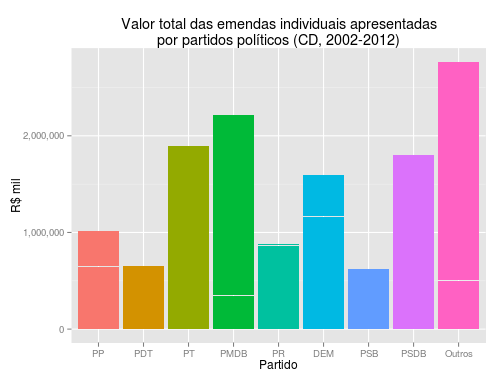
\includegraphics[scale=0.7]{c2g1.png}
	\caption{Total (em R\$ mil) de emendas apresentadas por partido político na Câmara dos Deputados entre 2002 e 2012.}
	\label{fig:c2g1}
\end{figure}

Muitos parlamentares de um partido tendem, por exemplo, a destinar recursos do governo federal para as prefeituras ou organizações sediadas nas capitais ou grandes municípios de seus estados. Por outro lado, para os menores municípios é comum que apenas um parlamentar de um único partido se preocupe em enviar recursos. Dessa forma, a distribuição dos valores que os partidos enviam aos municípios é bastante assimétrica e os maiores municípios recebem proporcionalmente mais recursos do partido do que os menores municípios. 55\% do total valor total de emendas individuais apresentadas é destinada a municípios com mais de 50 mil habitantes, um terço para municípios entre 10 e 50 mil habitantes e apenas 11\% aos menores municípios, com menos de 10 mil habitantes.

Se a suspeita teórica de que o resultado da eleição para prefeito e a decisão dos parlamentares ao emendar o orçamento são funções de um mesmo conjunto de variáveis observáveis e não observáveis (apoio eleitoral do partido no município, reputação, etc) for verdadeira, então devemos esperar correlação positiva entre tais variáveis. Entretanto, um dos aspectos problématicos da presente análise é como medir $Y_{i}$. As variáveis dependentes do Capítulo~\ref{cap:eleicoes} eram bastante mais simples e de fácil interpretação do que as variáveis deste capítulo. Em primeiro lugar, porque a freqência de zeros no numerador para as variáveis aqui utlizadas é muito grande. Dos mais de 32 mil casos válidos, formados por um combinação de partido ($p$), município ($m$) e eleição ($t$), em 83\% o valor de $Y_{i}$ é zero para todas as modalidades de aplicação. Em outras palavras, em 83\% dos casos em que o partido venceu as eleição para prefeito ou ficou em segundo colocado nenhum parlamamentar do partido, em nenhum dos três anos antes da próxima eleição municipal, destinou recursos ao município por nenhuma modalidade de aplicação. Quando consideradas apenas as transferências diretas para prefeitura, o percentual de zeros sobe para quase 85\%. Para as ESFLs a situação é ainda mais crítica e somente 1,7\% são não nulos. Dado que a operacionalização do desenho de regressão descontínua requer a exclusão das observações para obter identificação correta do efeito causal da vitória eleitoral, a existência de muitos casos com zero é bastante comprometedora. 

Note-se que o grande número de casos com $Y_{i}=0$ é resultado dos limites formais para emendas individuais no processo orçamentário. Vamos supor que os parlamentares de um partido tenham interesse em distribuir igualmente recursos entre $n$ municípios um valor $v$ via emendas individuais. Entretanto, $n*v$ é maior que teto permitido para emendas individuais para este partido no orçamento. Dessa forma, os parlamentares elegem $k$ municípios dentre os $n$ para beneficiarem. A consequência imediata desta restrição é que ao medir $Y_{i}$ para os demais $n-k$ municípios não beneficiados por este partido obtêm-se o valor zero quando a esperança para esta variável é diferente de zero ($E[Y_{i}]>0$).

A existência de algumas observações em que $Y_{i}=0$ mesmo quando $E[Y_{i}] \ne 0$ foi a razão pela qual no primeiro capítulo diversos partidos foram excluídos da análise dos efeitos da vitória no município nas eleições para senador, governador e presidente. Infelizmente, neste capítulo não há um critério objetivo que consiga separar os casos em que $Y_{i}=0$ e $E[Y_{i}]=0$ dos casos em que $Y_{i}=0$ e $E[Y_{i}] \ne 0$. Além disso, os casos com zero não estão igualmente distribuídos entre os grupos de tratamento. Quando consideradas as transferências diretas a prefeituras, aproximadamente 53\% das unidades em que $Y_{i}=0$ são não tratadas. Quando consideradas somente as transferências a ESFLs, a distribuição metade dos casos com zero está em cada um dos grupos.

Assim, a solução encontrada é produzir a análise com e sem os casos da variável dependente igual a zero, tendo em vista que a inclusão  dos casos com $Y_{i}=0$ favorece a produção de resultados positivos, posto que há mais unidades não tratadas com valores nulos do que unidades tratadas.

\begin{figure}[htp]
	\centering
	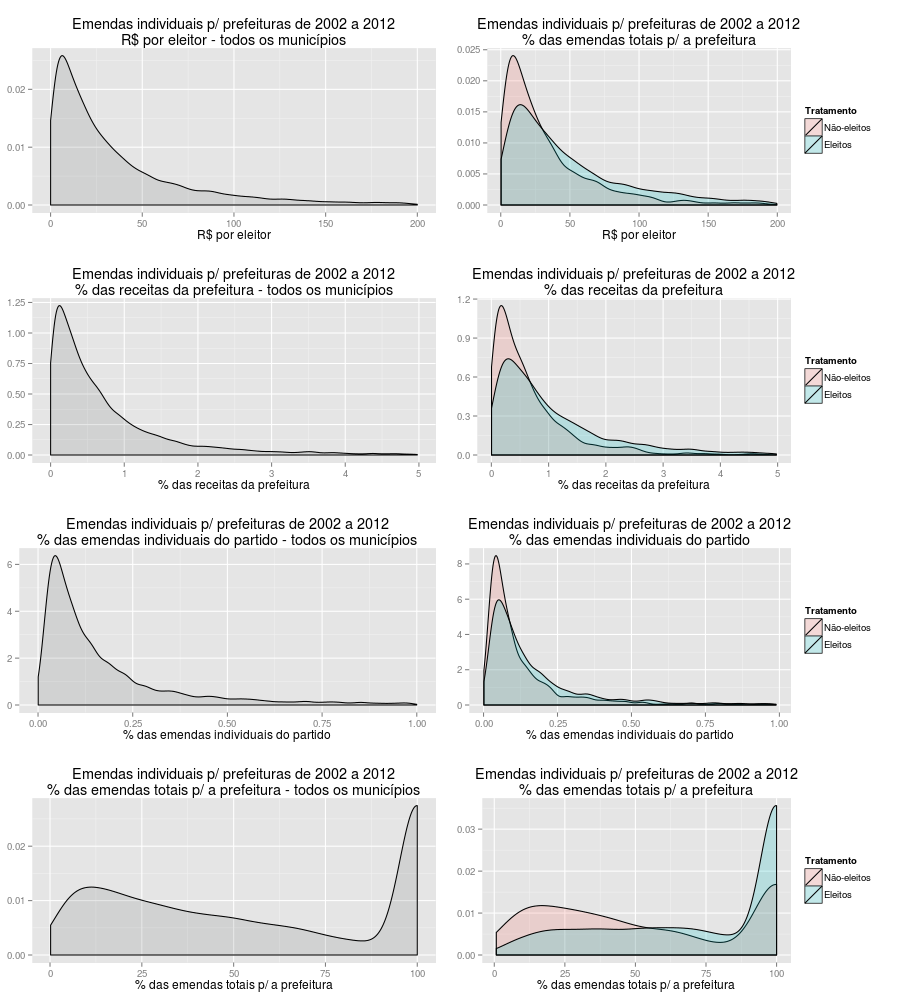
\includegraphics[scale=0.45]{c2g2.png}
	\caption{Distribuição das quatro medidas da variável dependente $Y_{i}^{pref}$ -- transferências diretas a prefeituras cuja origem são emendas individuais de deputados federais -- entre 2002 e 2012. Os gráficos à esquerda contemplam todos os municípios, inclusive os que não integram a análise. Os gráficos à direita da figura contém apenas os municípios incluídos na análise e separa-os por grupo de tratamento.}
	\label{fig:c2g2}
\end{figure}

Além do problema do grande número de zeros, a escolha do denominador da variável tem muito impacto sobre sua distribuição. A Figura~\ref{fig:c2g2} apresenta a distribuição das quatro diferentes maneiras de medir $Y_{i}^{pref}$. De um lado está a distribuição para a totalidade de partidos ($p$) e municípios ($m$) entre 2000 e 2012, não importanto a posição do partido na eleição municipal ou mesmo se o partido concorreu. Do outro estão os casos em que o partido terminou entre os dois primeiros colocados na disputa para prefeito e, portanto, que compõem o conjunto de dados da análise. Este último conjunto está separado por grupo de tratamento. Estão excluídos os casos em que $Y_{i}^{pref}=0$ ou apresenta valores extremos. A inclusão dos casos de $Y_{i}^{pref}=0$ inviabilizaria a observação gráfica da variação dos demais valores.

É possível notar que a primeira medida de $Y_{i}^{pref}$, R\$ por eleitor, é bastante assimétrica e tem distribuição semelhante para os dois conjuntos de dados. A grande maioria das prefeituras que se beneficiam de alguma emenda parlamentar recebem até R\$ 100,00 por eleitor e há poucos casos extremos. Dentre as observações incluídas da análise, vemos claramente que há mais observações não tratadas para o menores valores de $Y_{i}$. Por outro lado, a partir de aproximadamente R\$ 30,00 por eleitor, há mais observações tratadas do que não tratadas. Este é um forte indicativo de que os parlamentares tendem a enviar mais recursos a municípios nos quais o partido venceu as eleições para prefeito. É preciso, porém, avançar na análise e estimar corretamente os efeitos causais da vitória eleitoral com um desenho de regressão descontínua.

Algo semelhante ocorre quando a variável dependente representa a proporção das emendas individuais nas receitas da prefeitura ou como proporção do total de emendas individuais apresentadas pelo partido e que beneficiam municípios. Vemos que a soma das emendas individuais introduzidas no orçamento por um partido raramente representa mais de 2\% das receitas municipais na grande maioria dos municípios. Também é possível notar que, em geral, a soma das emendas para um município específico normalmente representa até 0.5\% da soma total das emendas individuais do partido. Para ambas as medidas de $Y_{i}^{pref}$ os valores mais baixos são mais frequentes nos casos em que o partido não venceu as eleições para prefeito, enquanto os valores mais altos são mais frequentes entre unidades tratadas.

Quando $Y_{i}^{pref}$ representa a participação das emendas individuais de um partido no total de emendas que beneficiam o município, porém, a variável tem um comportamento pouco usual. Em diversas situações a prefeitura será beneficiada por emendas de apenas um partido. Por esta razão, a variável têm, além de uma grande quantidade de zeros omitidos, muitas observaçoes em que $Y_{i}^{pref}=100$. O comportamento pouco usual desta variável pode provocar distorções nos resultados, uma vez que pode haver desequilíbrio entre os grupos de tratamento. De fato, 54\% dos casos em que $Y_{i}^{pref}=100$ pertencem ao grupo dos não tratados.

\begin{figure}[htp]
	\centering
	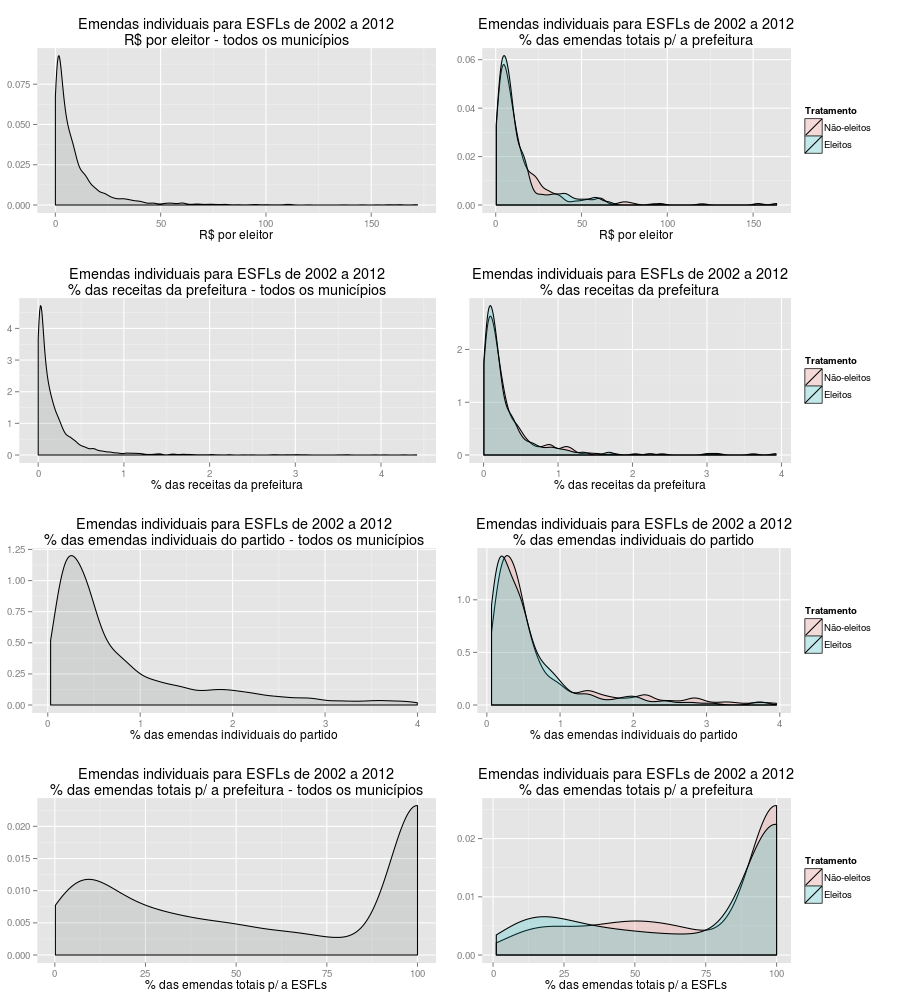
\includegraphics[scale=0.45]{c2g3.png}
	\caption{Distribuição das quatro medidas da variável dependente $Y_{i}^{esfl}$ -- transferências diretas a Entidades Sem Fins Lucrativos cuja origem são emendas individuais de deputados federais -- entre 2002 e 2012. Os gráficos à esquerda contemplam todos os municípios, inclusive os que não integram a análise. Os gráficos à direita da figura contém apenas os municípios incluídos na análise e separa-os por grupo de tratamento.}
	\label{fig:c2g3}
\end{figure}

A Figura~\ref{fig:c2g3} reproduz os gráficos para as quatro maneiras diferentes de medir $Y_{i}^{esfl}$. As distribuições são bastante semelhantes, com algumas diferenças importantes a se notar. A primeira delas é que mudam as faixas de valores em que as observações estão distribuídas. Para as duas primeiras medidas da variável, temos que a grande maioria dos casos se concentra em até R\$ 25 por eleitor e 1\% das receitas municipais. Por outro lado, a soma das emendas individuais de um partido para ESFLs de um município representam um valor maior do total de emendas individuais do partido para todas as ESFLs do país, posto que há menos emendas que beneficiam ESFLs do que emendas que beneficiam prefeituras.

O segundo aspecto importante a se notar é que as curvas entre os diferentes grupos de tratamento têm distribuição bastante semelhante, um importante indicativo de que talvez o tratamento não tenha efeito, nem positivo, nem negativo, sobre as decisões do parlamentares em relação à destinação de recursos para ESFLs.

Por fim, é importante observar que as três primeiras medidas têm valores extremos tanto para $Y_{i}^{pref}$ quanto $Y_{i}^{esfl}$. Esses valores extremos são, na maioria das vezes, consequência da escolha do denominador e poderiam provocar distorções no resultado. Enquanto no primeiro capítulo a amplitude das variáveis dependentes era bastante clara e limitada, de 0\% a 100\%, neste capítulo as variáveis estão limitadas a 0\% por um lado mas podem assumir valores anormais no outro extremo da distribuição. A solução dada a este problema foi excluir todos os valores acima de três desvios padrão da distribuição nas medidas que não têm limite superior, ou seja, qualquer valor fora dos primeiros 99,73\% da distribuição dessas variáveis.

A opção por um desenho de regressão descontínua está fundamentada na suspeita de que as decisões dos parlamentares sobre suas emendas individuais, o desempenho do partido nas eleições para prefeito e o próprio tratamento são resultado de um mesmo conjunto de fatores não observáveis ou conhecidos. Espera-se, portanto, que tais variáveis esteja correlacionadas entre si. Dito de outra forma, se os deputados federais utilizam estrategicamente as emendas individuais para obter votos, devemos observar uma correlação positiva entre o volume de recursos destinados pelos parlamentares de um partido a um município e o desempenho do partido nas eleições municipais.

A expectativa de uma correlação positiva se estende também a transferências a Entidades Sem Fins Lucrativos. Apesar de esperar que o tratamento tenha efeito negativo na decisão dos parlamentares enviarem recursos a ESFL no município, se espera que os parlamentares privilegiem os municípios nos quais o partido têm mais votos. Por esta razão, é fundamental um desenho de pesquisa que identifique corretamente o efeito do tratamento e possa separar a correlação entre as variáveis do impacto de vencer as eleições para prefeito.

\begin{figure}[htp]
	\centering
	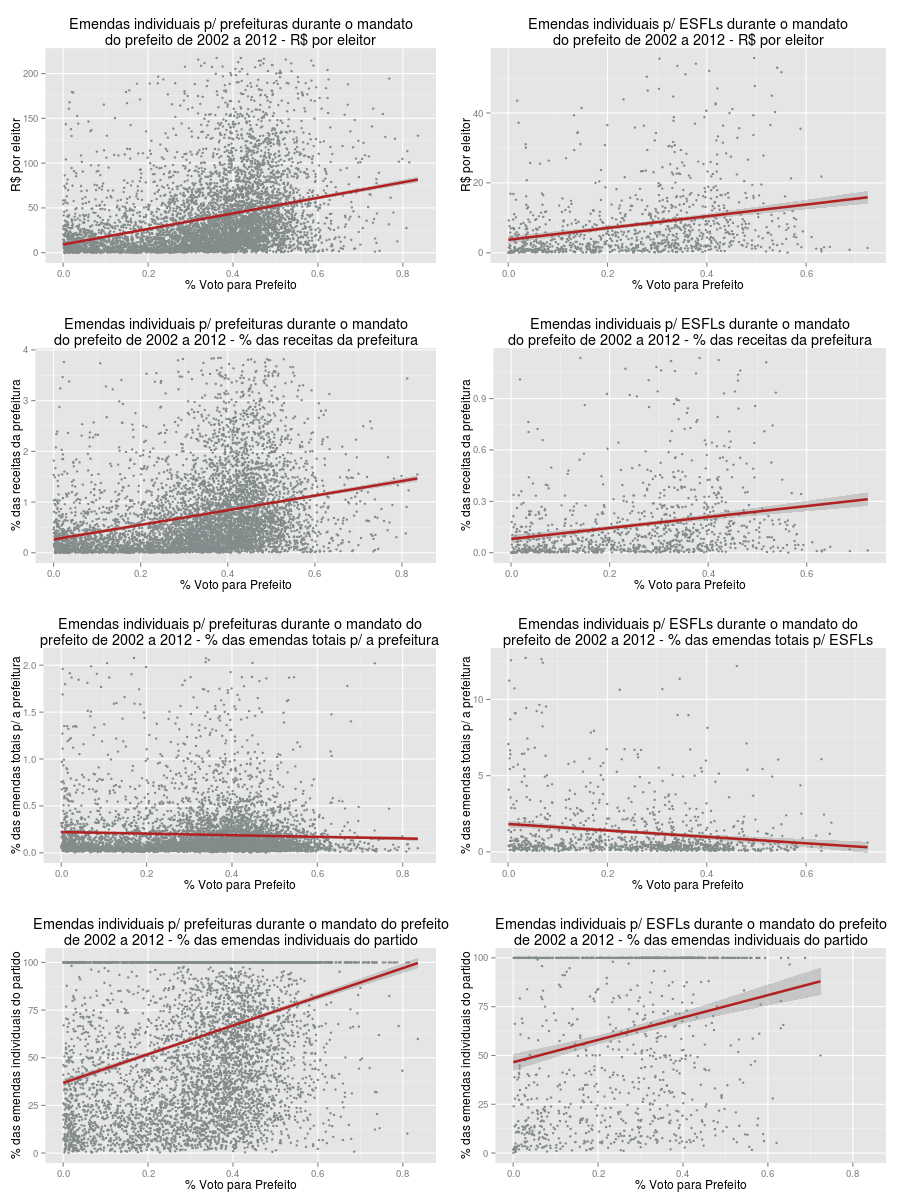
\includegraphics[scale=0.45]{c2g4.png}
	\caption{Distribuição das quatro medidas da variável dependente $Y_{i}^{pref}$ e $Y_{i}^{esfl}$ -- transferências diretas a prefeituras e ESFLs cuja origem são emendas individuais de deputados federais -- entre 2002 e 2012 pelo voto nas eleições para prefeito anteriores.}
	\label{fig:c2g4}
\end{figure}

A Figura~\ref{fig:c2g4} apresenta a distribuição das quatro medidas de $Y_{i}^{pref}$ e $Y_{i}^{esfl}$ pelo voto nas eleições para prefeito anterior à apresentação das emendas. São incluídos todos os casos em que a soma das emendas individuais do partido para o município são maiores do que zero e o partido concorreu nas eleições para prefeito. A linha vermelha em cada um dos gráficos descreve uma relação linear entre as variáveis.

A inclinação das retas que sintetizam as distribuições apresentadas têm o mesmo sinal para emendas que beneficiam prefeituras ou Entidades Sem Fins Lucrativos. A relação do desempenho do partido nas eleições para prefeito com $Y_{i}$ é positiva quando esta última representa a soma das emendas individuais de um partido para um município pelo total de eleitores do município, pela receita municipal ou como proporção das emendas de todos os partidos ao município. É bastante claro, portanto, que existe um conjunto de fatores não observáveis que explica ambas as variáveis. Quando a variável dependente $Y_{i}$ é construída como o total de emendas individuais do partido para um município sobre o total de emendas individuais do partido para todos os municípios, parece não haver relação da variável com os votos que o partido recebeu na eleição municipal. A reta que descreve a relação tem inclinação negativa, mas é praticamente horizontal.

Mais importante do que observar a correlação entre as duas variáveis retratadas nos gráficos da Figura~\ref{fig:c2g4} é notar que a dispersão de $Y_{i}$ é bastante alta, seja quando o partido teve bom ou mau desempenho nas eleições para prefeito. É de se esperar, assim, que próximo à fronteira de atribuição do tratamento definida por $\tau_{i}=0$ a dispersão de $Y_{i}$ também seja grande. Haverá casos em que as somas das emendas individuais apresentam valores altos e casos em que este somatório apresenta valores bastante baixos (além dos inúmeros zeros) mesmo ao selecionar apenas eleições competitivas e definidas por uma margem estreita de votos, em que primeiro e segundo colocados têm desempenhos semelhantes e melhores do que os demais oponentes.

\begin{figure}[htp]
	\centering
	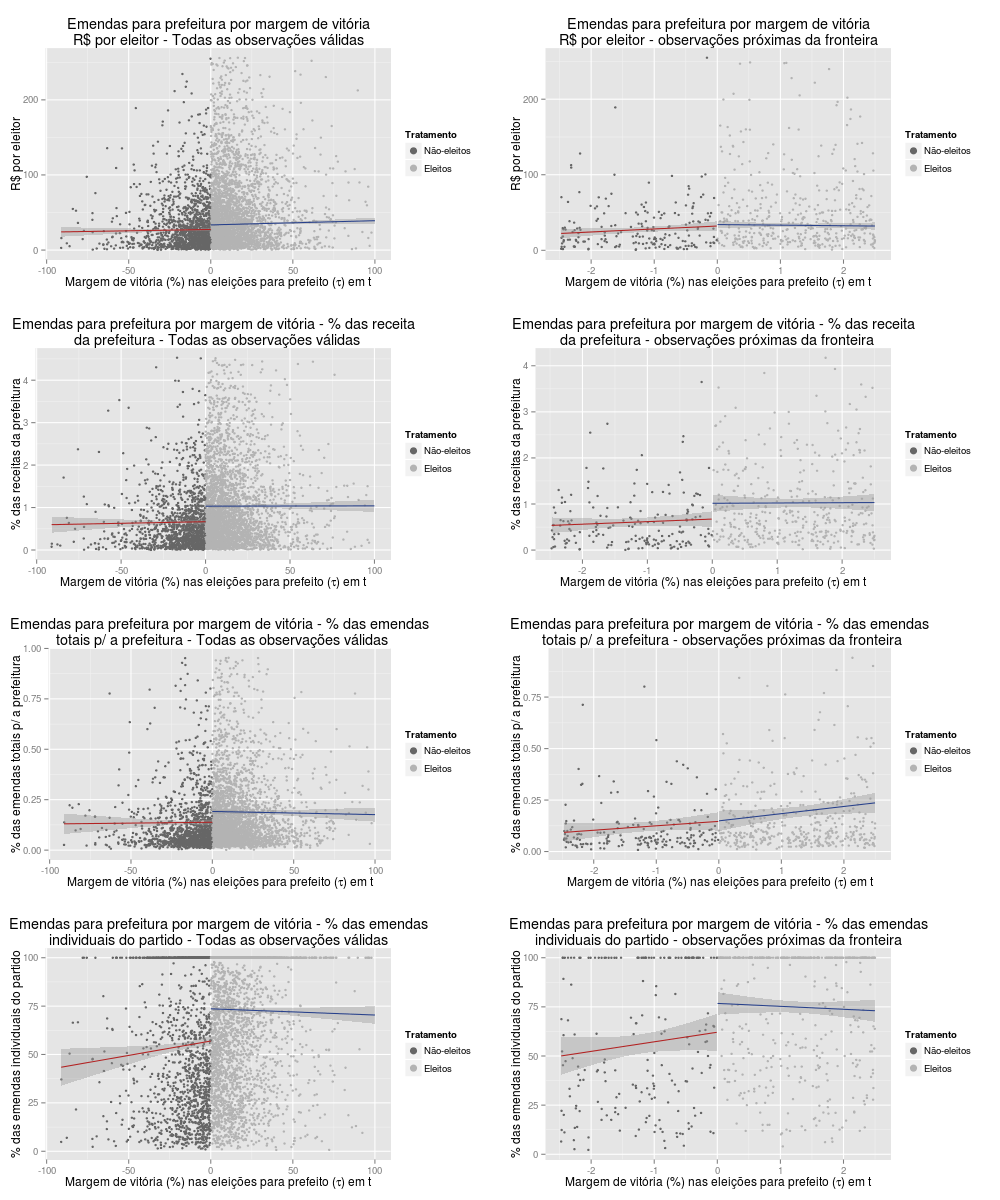
\includegraphics[scale=0.45]{c2g5.png}
	\caption{Distribuição das quatro medidas da variável dependente $Y_{i}^{pref}$ -- transferências diretas a prefeituras cuja origem são emendas individuais de deputados federais -- entre 2002 e 2012 por margem de vitória para prefeito.}
	\label{fig:c2g5}
\end{figure}

A Figura~\ref{fig:c2g5} apresenta as quatro medidas de $Y_{i}^{pref}$ por margem de vitória. Para cada medida há dois gráficos, um com todos os casos em que o partido $p$ terminou a eleição para prefeito em primeiro ou segundo lugar e um para todos os casos que atendem à restrição da margem de vitória $-\Delta \leq \tau \leq \Delta$, com $\Delta=2,5\%$. Em todos os gráficos os pontos cinza escuro são as unidades não tratadas, enquanto os pontos azuis claros são as unidades tratadas. As retas vermelha e azul são funções lineares que descrevem as unidades em cada um dos grupos de tratamento, respectivamente. 

Note-se que o exercício da Figura~\ref{fig:c2g5} se aproxima do procedimento adotado em um desenho de regressão descontínua. O pressuposto adotado na análise é que para margens próximas a zero a probabilidade de uma observação ser tratada é a mesma de não ser tratada. Dada a forma com que este problema foi construíudo, nos gráficos em que $\Delta \leq 100\%$, a posição das observações no eixo das abscissas é resultado, pelo menos em teoria, de um conjunto de fatores não observáveis, enquanto nos gráficos em que $\Delta \leq 2,5\%$, a posição das observações no mesmo eixo é quase aleatória. As observações em que $Y_{i}^{pref}=0$ foram excluídas

\begin{figure}[htp]
	\centering
	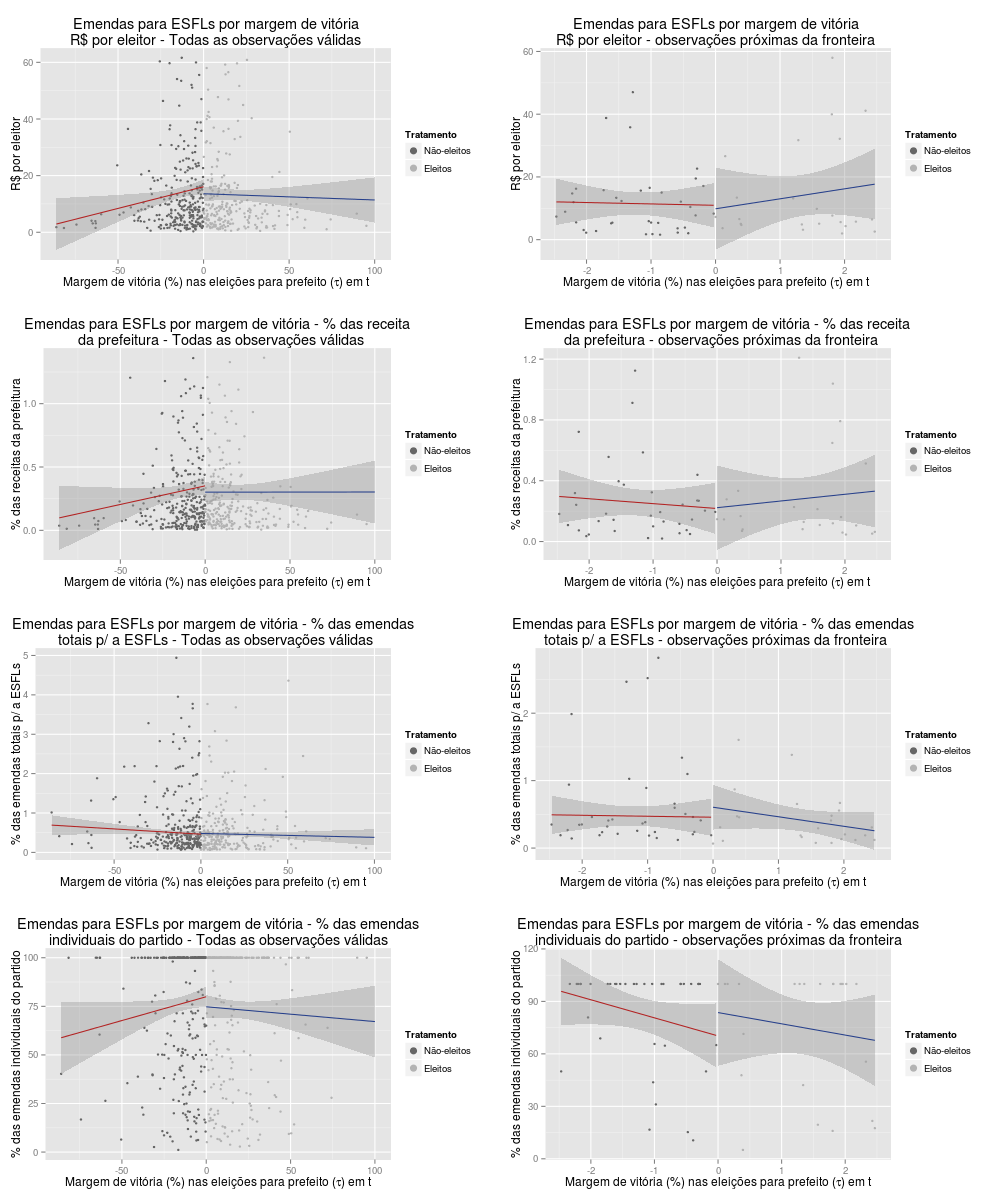
\includegraphics[scale=0.45]{c2g6.png}
	\caption{Distribuição das quatro medidas da variável dependente $Y_{i}^{esfl}$ -- transferências diretas a ESFLs cuja origem são emendas individuais de deputados federais -- entre 2002 e 2012 por margem de vitória para prefeito.}
	\label{fig:c2g6}
\end{figure}

A Figura~\ref{fig:c2g6} apresenta gráficos semelhantes para $Y_{i}^{esfl}$. A principal diferença em relação aos gráficos da Figura~\ref{fig:c2g5} é o número bastante reduzido de observações para todas as medidas da variável. As consequências do número baixo de observações para a análise são bastante visíveis nos gráficos em que $\Delta$ é limitado: os intervalos de confiança para a reta de regressão que descreve os pontos é bastante maior para $Y_{i}^{esfl}$ do que para $Y_{i}^{pref}$. 

A forma como os resultados são estimados no capítulo, mesmo quando o efeito causal $\rho$ for estimado como descontinuidade em uma função linear, são um pouco diferentes das retas apresentas nas Figura~\ref{fig:c2g5} e ~\ref{fig:c2g6}. Entretanto, já podemos ter uma expectativa clara dos resultados para cada uma da variáveis e das medidas de cada variável. A depender do denominador utilizado na construção $Y_{i}^{pref}$, há, aparentemente, diferenças entre os grupos de tratamento. Para $Y_{i}^{esfl}$ podemos esperar resultados nulos, dado que os intervalos de confianças são demasiadamente altos.

Antes de avançar para a estimação dos efeitos causais, $\rho$, convém examinar, como no primeiro capítulo, se o desenho de pesquisa está adequadamente construído e se não há efeito do tratamento em variáveis anteriores ou contemporâneas à sua ocorrência.

\subsection{Testando a validade do Desenho de Regressão Descontínua: o não-impacto das eleições para prefeito nas decisões passadas dos deputados federais}

O principal risco para o desenho de regressão descontínua é a possibilidade de desequilíbrio em covariáveis entre unidades tratadas e não tratadas. Se estas covariáveis estiverem correlacionadas com a variável resposta ($Y_{i}$), então o efeito estimado do tratamento será viesado.

No Capítulo~\ref{cap:eleicoes} analisamos o impacto da vitória nas eleições para prefeito nos resultados eleitorais passados do partido e vimos que não há diferenças entre unidades tratadas e não tratadas quanto a esta variável. Em particular, já sabemos que vencer as eleições para prefeito não afeta o desempenho anterior do partido para deputado federal ou prefeito, ou mesmo o total de votos que o partido recebeu para vereador simultaneamente à eleição que definiu tratados e não tratados. Este resultado é bastante importante pois não apenas o desempenho retrospectivo, mas também qualquer outra variável passada ou contemporânea à definição do tratamento, por construção, não pode ser afetada pelo tratamento. A existência de efeito de $d_{i}$ sobre tais variáveis (representadas novamente por $O_{i}$) comprometeria a análise do desenho de regressão descontínua proposto\footnote{O Capítulo~\ref{cap:financiamento} retoma o tema do desequiblíbrio entre os grupos de tratados e não tratados e apresenta problemas inicialmente não discutidos nesta seção. Como se observará adiante, há uma variável para a qual o desequilíbrio entre tratados e não tratados é mais sério: as receitas de campanha para prefeito. Sistematicamente, partidos vitoriosos arrecadaram mais do que partidos derrotados, mesmo quando são comparados apenas os casos nos quais a margem de vitória tende a zero. O Capítulo~\ref{cap:financiamento} trata apenas deste assunto e revê os resultados dos três primeiros capítulos à luz deste problema.}.

Portanto, os testes realizados no capítulo~\ref{cap:eleicoes} tornam bastante mais confiáveis os resultados que são apresentados neste capítulo. O resultado eleitoral passado, a margem de vitória nas eleições para prefeito e as decisões dos parlamentares são, pelo menos em teoria, funções do mesmo conjunto de variáveis não observáveis ($A_{i}$). Assim, para que o resultado possa ser estimado sem viéis, é fundamental que o tratamento tenha independência em relação a tais fatores quando $\Delta$ é próximo de zero.

Ainda assim, especificamente para este capítulo, convém examinar se o desenho de pesquisa proposto tem validade quando $O_{i}$ representa as decisões passadas sobre emendas individuais por parte dos deputados federais de um partido. Infelizmente, para este trabalho não foram coletados os valores das emendas individuais apresentadas pelos deputados federais anteriores a 2002. Dessa maneira, é possível testar o efeito da vitória para prefeito nas decisões dos partidos no Congresso para as eleições municipais de 2004 e 2008. Fica de fora, portanto, a eleição de 2000, que terá como teste de validação apenas os resultados já apresentados. Vale lembrar que a eleição de 1996 está excluída da análise e não há razão para nos preocuparmos com ela agora.

\begin{figure}[htp]
	\centering
	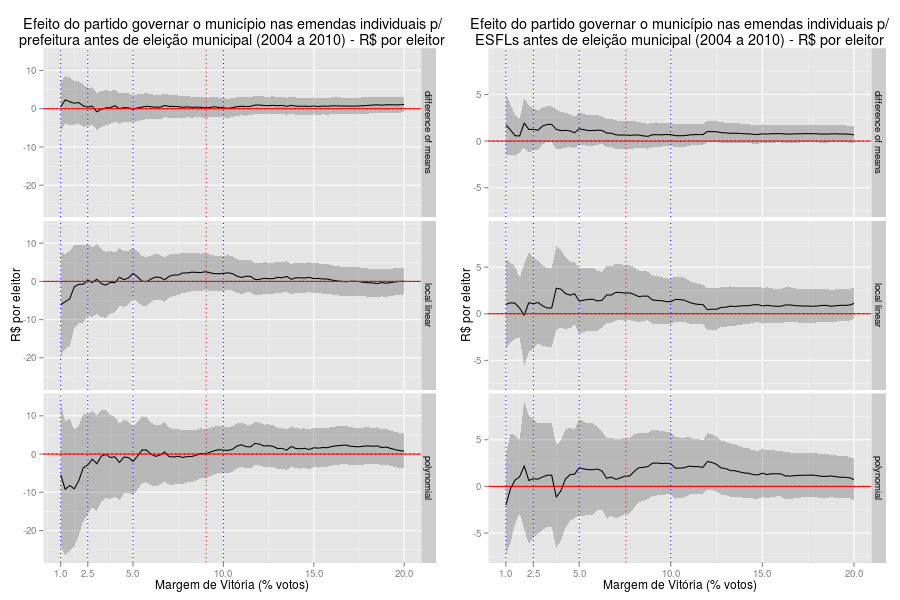
\includegraphics[scale=0.45]{c2g7.png}
	\caption{Efeito do Tratamento nas emendas individuais apresentadas por parlamentares do partido (em R\$ por eleitor) nos três últimos anos do mandato de prefeito anterior à eleição municipal por margem de vitória para prefeito (2002 a 2008).}
	\label{fig:c2g7}
\end{figure}

$O_{i}$ assume nesta seção as diferentes medidas para as duas principais variáves adotadas no capítulo. A primeira delas é simplesmente o total em emendas apresentas por deputados federais que do partido $p$ que beneficiam diretamente a prefeitura ou as ESFLs do município $m$ nos dois últimos anos antes da eleição municipal e no próprio ano eleitoral $t$ por eleitor apto em $t$. A Figura~\ref{fig:c2g7} apresenta o efeito da vitória nas eleições de 2004 e 2008 para prefeito para $O_{i}$ medida desta maneira, excluindo os municípios em que $O_{i}=0$. Para cada um dos gráficos desta seção há um gráfico semelhante no Anexo que inclui as observações com $O_{i}=0$ e cujos resultados comento no texto.

Não há evidências de que o resultado nas eleições para prefeito afeta as decisões passadas dos deputados federais em relação a emendas individuais. Não há diferenças relevantes com a exclusão das observações em que $O_{i}=0$, cujos resultados constam do Anexo. O efeito estimado representa a diferença entre a média para cada grupo de tratamento do percentual em emendas individuais alocadas no município por eleitor. Por exemplo, uma diferença de R\$ 1,00 significaria que os deputados federais do partido alocam em média um real a mais por eleitor do total das emendas individuais aos municípios em que o partido venceu.

\begin{figure}[htp]
	\centering
	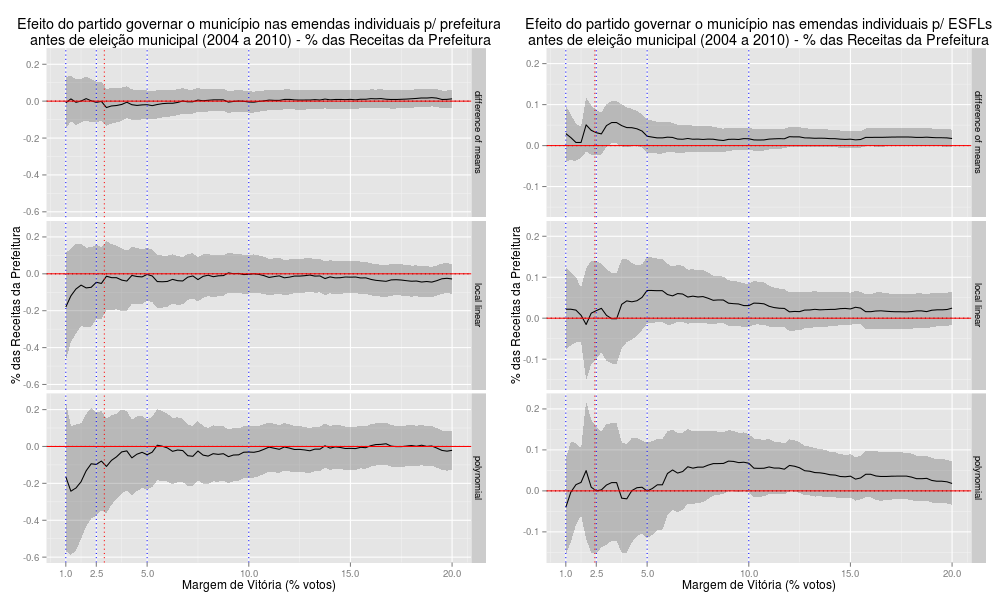
\includegraphics[scale=0.45]{c2g8.png}
	\caption{Efeito do Tratamento nas emendas individuais apresentadas por parlamentares do partido (como razão das receitas da prefeitura) nos três últimos anos do mandato de prefeito anterior à eleição municipal por margem de vitória p/ prefeito (2002 a 2008).}
	\label{fig:c2g8}
\end{figure}

Da mesma forma que no primeiro capítulo, quando tiver de apresentar com mais parcimônia os resultado, darei preferência à apresentação do efeito estimado como descontinuidade em uma regressão linear simples.

Na Figura~\ref{fig:c2g8}, repito o procedimento alterando o denominador utilizado para a construção de $O_{i}$. Neste caso, a variável representa o percentual de recursos beneficiando o município $m$ apresentados em emendas individuais do partido $p$ sobre o total de receitas municipais nos três últimos anos de mandato do prefeito antes da eleição municipal em $t$. Os resultados para esta medida convergem com o anterior e não por acaso: eleitorado e receitas municpais são função da população do município. Novamente o efeito estimado é nulo, não importando se os casos com $O_{i}=0$ são ou não omitidos e tampouco o estimador utilizado.

As Figuras ~\ref{fig:c2g9} e ~\ref{fig:c2g10} trazem os resultados do efeito do tratamento em $O_{i}$ quando esta variável é medida como total de emendas individuais de um partido que beneficiam um município em relação ao total de emendas individuais do próprio partido ou como total de emendas individuais de um partido que beneficiam um município em relação ao total de emendas de todos os partidos que beneficiam o município. Em ambos os casos os resultados para $O_{i}>0$ são nulos e não há efeito algum do tratamento, seja para transferências a prefeituras ou transferências ESFLs. Quando $O_{i}$ é a proporção de emendas de um partido sob o total de emendas do município e $O_{i} \geq 0$ (no Anexo), porém, há efeito do tratamento para margens próximas a zero para qualquer forma de estimar o efeito do tratamento $\rho$ quando as emendas são elaboradas em benefício das prefeituras.

\begin{figure}[htp]
	\centering
	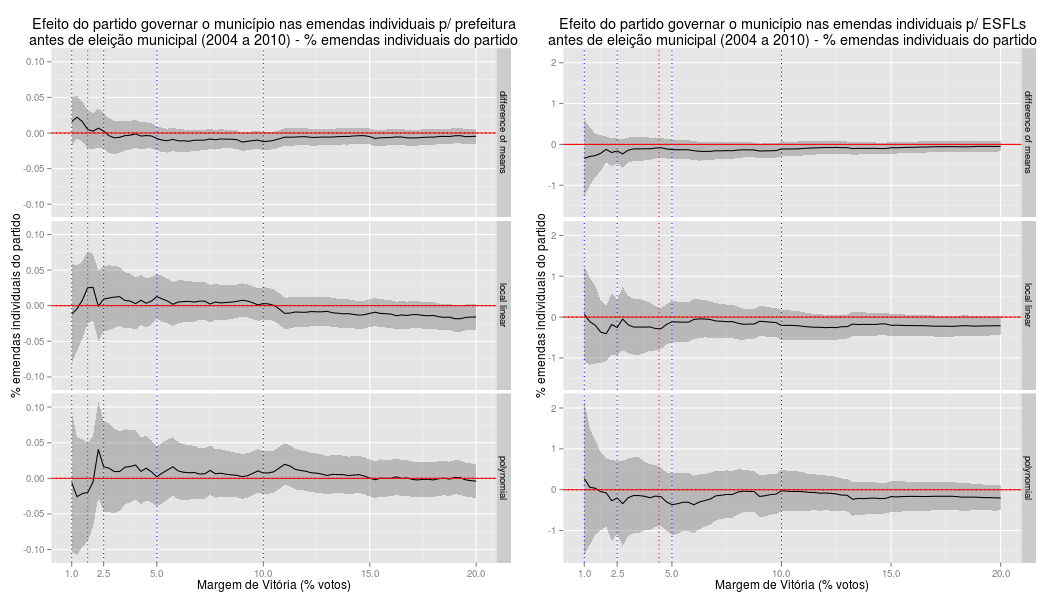
\includegraphics[scale=0.45]{c2g9.png}
	\caption{Efeito do Tratamento nas emendas individuais apresentadas por parlamentares do partido (como razão do total em emendas de todos os partidos para prefeitura ou ESFLs do município) nos três últimos anos do mandato de prefeito anterior à eleição municipal por margem de vitória para prefeito (2002 a 2008).}
	\label{fig:c2g9}
\end{figure}

É necessário refletir sobre este único resultado inesperado, sobre a direção do sinal e suas potenciais consequências. Esperamos que a existência de fatores não observáveis tenham como consequência o bom desempenho do partido entre eleições e também a maior probabilidade do partido beneficiar o município com emendas, independetemente dos resultados eleitorais nas eleições municipais. Entretanto, obsevarmos uma relação negativa entre vencer a eleição e a probabilidade do município receber emendas do partido no passado. O viés do estimador tem, dessa forma, sinal contrário à expectativa do efeito do tratamento. Se há viés derivado do desequilíbrio nesta variável, ele torna mais difícil a obtenção de um resultado positivo.

\begin{figure}[htp]
	\centering
	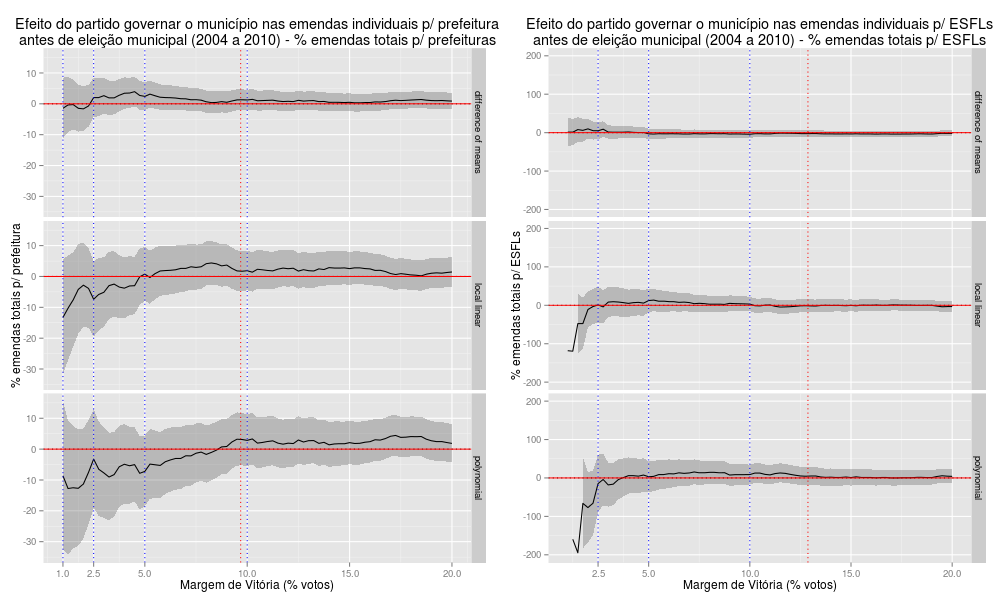
\includegraphics[scale=0.45]{c2g10.png}
	\caption{Efeito do Tratamento nas emendas individuais apresentadas por parlamentares do partido (como razão do total de emendas do partido para prefeituras ou ESFls) nos três últimos anos do mandato de prefeito anterior à eleição municipal por margem de vitória para prefeito (2002 a 2008).}
	\label{fig:c2g10}
\end{figure}

A razão mais provável para o desequilíbrio é que a maioria dos casos em que $O_{i}=0$ para esta medida são casos não tratados, ou seja, são municípios nos quais o partido perdeu a eleição em $t$. Para $\Delta \leq 2,5$ há 2,5\% mais casos não tratados. Como para estes casos $O_{i} \ne E[O_{i}]$, o desequilíbrio pode ser apenas resultado da incapacidade de medir as preferências de deputados sobre todos os municípios em um contexto em que apenas algumas prefeituras são beneficiadas pelos parlamentares no Congresso Nacional. É mais seguro, como já se havia indicado, priorizar a comparação entre municípios que recebem emendas em vez de incluir todos os municípios. A seguir, vamos observar os resultados deste capítulo. 

\section{Emendas individuais ao Orçamento, prefeitos e ESFLs}

O objetivo deste capítulo é testar se as eleições para prefeito afetam a decisão dos deputados federais no processo orçamentário. Este problema pode ser lido também da seguinte maneira: o partido que governa o município influencia a decisão dos parlamentares na Câmara dos Deputados em relação às emendas individuais? O argumento central do capítulo é que os deputados federais destinam recursos preferencialmente a prefeitos de seu próprio partido e não necessariamente para as localidades nas quais tiveram retrospectivamente mais votos, tal como costumam apontar trabalhos que evidenciam o voto pessoal e a \emph{conexão eleitoral} como aspectos centrais do sistema politico brasileiro. Em outras palavras, espera-se produzir evidências de que o uso estratégico das emendas individuais na Câmara dos Deputados, antes de revelar a atuação particularista dos deputados federais, aponta para a ação coordenada dos políticos brasileiros dentro das organizações partidárias e entre diferentes níveis de governo. Talvez a conexão que de fato importe seja a \emph{conexão partidária}, e não a \emph{conexão eleitoral}.

Como apontado anteriormente no capítulo, devemos esperar que os municípios beneficiados pelas emendas individuais dos parlamentares de um partido sejam também aqueles nos quais o partido tenha maior expectativa de votos nas eleições municipais, estaduais e nacionais. Por esta razão, é necessário adotar uma estratégia analítica que permita identificar adequadamente o impacto de vencer as eleições municipais -- ou o impacto do partido governar o município -- no total de emendas destinadas ao município por parlamentares de um partido. 

Nesta seção, apresento os resultados e os efeitos estimados adotando como variável dependente tanto a soma das emendas individuais apresentadas por parlamentares de um partido que beneficiem a prefeitura de um município quanto a soma das emendas individais que beneficiem um conjunto de ESFLs situadas no município. Ambas as variáveis são medidas de mais de uma maneira, como já debatido anteriormente. Inicio a seção analisando emendas individuais na Câmara dos Deputados que beneficiem diretamente as prefeituras dos municípios. 

\subsection{Emendas individuais ao Orçamento e prefeitos: \emph{conexão partidária}} 

Deputados federais privilegiam prefeituras de municípios governados pelos próprios partidos ao apresentar emendas individuais ao orçamento? Os gráficos da Figura~\ref{fig:c2g11} apontam que, pelo menos a partir das eleições municipais de 2000, sim. Há um claro efeito do partido governar o município na decisão dos parlamentares quando $Y_{i}^{pref}$ representa a soma das emendas individuais que beneficiam a polulação por eleitor ou como proporção das receitas municipais. Em ambos os casos, apenas observações com $Y_{i}^{pref}>0$ foram utilizadas e os gráficos que incluem observações com $Y_{i}^{pref} \geq 0$ estão no Anexo.

Para a primeira medida apresentada, o efeito do tratamento $\rho$ é diferente de zero para qualquer estimador escolhido para margens de vitória próximas a zero. Adotando a margem de 2,5\% como referência e estimando $\rho$ como um descontinuidade em uma função linear, temos um efeito de R\$ 23,00 por eleitor. Ou seja, esperamos que os deputados federais de um partido destinem à prefeitura de um município R\$ 23,00 a mais por cidadão apto a votar em municípios governados pelo próprio partido em relação a municípios governados por outra agremiação. Um município de pequeno porte, por exemplo, que tehna 5 mil eleitores, deve receber em média R\$ 115 mil reais a mais de um partido, valor nada desprezível dado padrão das emendas na Câmara dos Deputados.

\begin{figure}[htp]
	\centering
	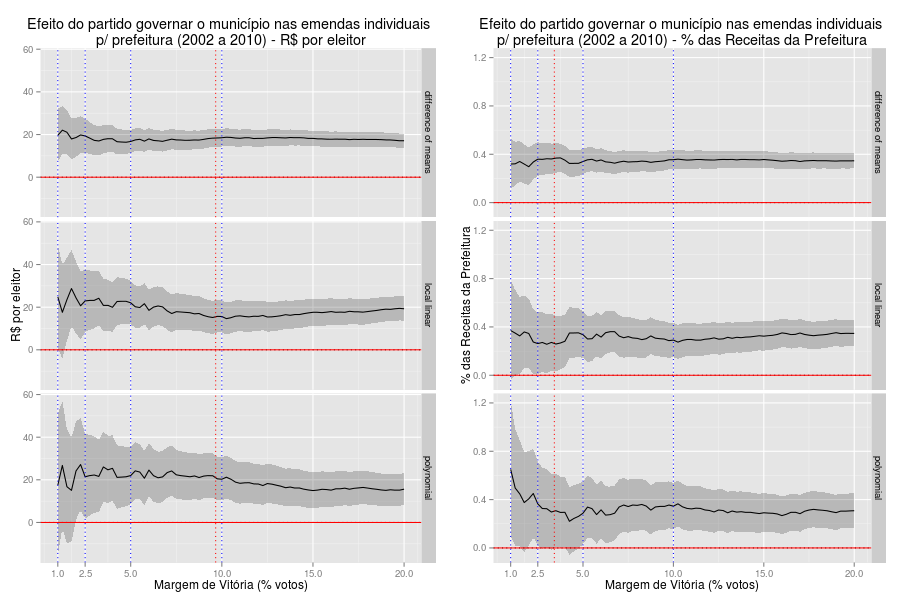
\includegraphics[scale=0.45]{c2g11.png}
	\caption{Efeito do Tratamento nas emendas individuais apresentadas por parlamentares do partido (R\$ por eleitor ou como razão das receitas do município) nos três últimos anos do mandato de prefeito por margem de vitória (2000 a 2012).}
	\label{fig:c2g11}
\end{figure}

Quando $Y_{i}^{pref}$ representa a razão entre as emendas individuais de um partido para a prefeitura de um município e as receitas totais do município, o efeito do tratamento também é diferente de zero para margens de vitória baixas. Mesmo ao estimar $\rho$ como descontinuidade em uma função polinomial, para $\Delta \leq 5\%$ o p-valor da estimativa do efeito do tratamento fica abaixo de 5\% em diversos momentos. Para $\rho$ estimado com uma função linear, o efeito é claramente diferente de zero para margens de vitórias mais baixas e no ponto $\Delta \leq 2,5\%$ o efeito estimado é de 0,26\%. Assim, prefeitos de um partido podem esperar receber mais recursos como proporção das receitas da prefeitura de parlamentares aliados do que prefeitos de outros partidos.

No Anexo apresento também os resultados incluindo $Y_{i}^{pref}=0$. Há duas diferenças fundamentais em relação aos resultados apresentados. A primeira delas é que o efeito é diferente de zero para praticamente qualquer margem de vitória ou forma de estimar o efeito causal ($\rho$), inclusive margens bastante próximas a zero. Ou seja, o gráfico não chega a cruzar nenhuma vez a linha vermelha para o conjunto de pontos apresentadosm, o que reforça o resultado positivo acima encontrado. A segunda diferença é que os efeitos estimados são menores. Para $\Delta \leq 2,5\%$, temos $\rho=$ R\$ 8,00 por eleitor ou $\rho=$ 0,12\% das receitas municipais. Ao aumentar o número de casos $Y_{i}^{pref}=0$, a queda na magnitude do efeito é absolutamente normal.

Essas duas primeiras medidas de $Y_{i}^{pref}$ são bastante úteis por levarem no denominador valores proporcionais ao tamanho dos municípios. Por esta razão é importante observar os resultados para as duas outras medidas de $Y_{i}^{pref}$, que são, respectivamente, o total de emendas individuais de um partido como proporção do total de emendas individuais de qualquer partido para um município, ou como proporção do total de emendas individuais do partido na Câmara dos Deputados (que beneficiem quaisquer municípios).

A Figura~\ref{fig:c2g12} apresenta o efeito estimado do tratamento em $Y_{i}^{pref}$ para ambas as medidas, excluindo os casos em que $Y_{i}^{pref}=0$. O efeito do tratamento para a razão do total destinado ao município pelo partido do prefeito sobre o total de emendas que beneficiam o município segue os resultados já apresentados. $\rho$ é diferente de zero para todas as margens menores ou iguais a qualquer valor no intervalo entre 2,5\% e 5\% quando estimado como descontinuidade em uma função linear ou polinomial. Para a referência adotada na análise ($\Delta \leq 2,5\%$ e função linear), o efeito estimado é de aproximadamente 17,7\%, ou seja, a participação do partido do prefeito no total de emendas individuais que beneficiam o governo municipal é quase um quinto maior do que a participação dos demais partidos. A inclusão das observações com $Y_{i}^{pref}=0$ novamente contribui para que o resultado seja ainda mais persistente à redução da margem e para o mesmo ponto de referência o efeito estimado é um pouco mais alto, com $\rho=$ 19,4\%.

\begin{figure}[htp]
	\centering
	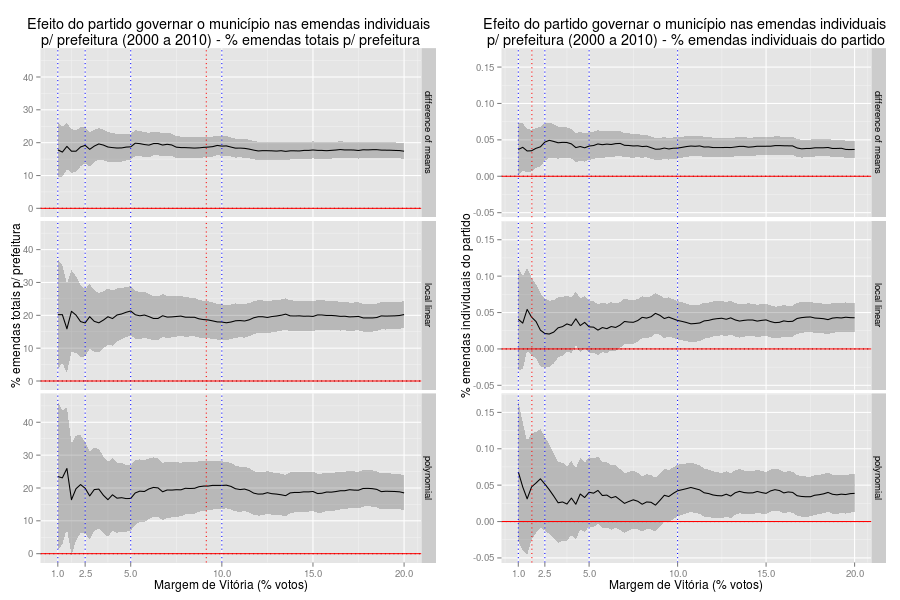
\includegraphics[scale=0.45]{c2g12.png}
	\caption{Efeito do Tratamento nas emendas individuais apresentadas por parlamentares do partido (como razão do total em emendas:1- de todos os partidos p/ prefeitura ou ESFLs do município; do partido p/ prefeituras ou ESFls) nos três últimos anos do mandato de prefeito por margem de vitória (2000 a 2012).}
	\label{fig:c2g12}
\end{figure}

Por outro lado, não é possível encontrar diferenças entre a proporção de emendas do partido para municípios governados pelo partido pelo total de emendas. O efeito não é diferente zero, com exceção para a estimação por diferença de médias. A inclusão das observações com $Y_{i}^{pref}=0$ altera bastante o resultado. Tal como as outras medidas de $Y_{i}^{pref}$, para qualquer margem ou estimador de $\rho$, o efeito é positivo e diferente de zero. Para $\Delta \leq 2,5\%$, o impacto do partido governar o município é $\rho=$ 0,017\%. Dado que normalmente um partido destina menos de 1\% de suas emendas para cada município, o efeito, ainda que pequeno, é relevante. Certamente, quando comparados com os demais resultados encontrados nesta seção, este é o menos expressivo.

O resultado combinado das diferentes formas de medir $Y_{i}^{pref}$ aponta na direção esperada: deputados federais privilegiam prefeituras governadas pelo seu próprio partido. Antes de avançar e reproduzir a análise para as emendas cujos beneficiários são as ESFLs, cabe analisar os possíveis efeitos heterogêneos do resultado encontrado. 

\subsection{Emendas individuais ao Orçamento e prefeitos: partidos no governo e na oposição e demais efeitos heterogêneos}

Um dos pressupostos adotados na presente análise é o de que os deputados federais apresentam emendas individuais ao orçamento de acordo com suas preferências alocativas e sem considerar a probabilidade das emendas serem ou não executadas pelo pode Executivo. Contudo, e se parlamentares em partidos aliados à presidência tiverem expectativas diferentes quanto à aprovação de suas emendas em comparação aos parlamentares em partidos de oposição? Se os parlamentares conhecem as chances de suas emendas serem executadas, e se as chances variarem dependendo da posição em relação ao governo federal, então devemos esperar comportamentos diferentes entre parlamentares governistas e oposicionistas.

Uma das expectativas que os parlamentares podem ter é que o governo federal também leva em consideração qual é o partido no governo municipal para decidir se executa ou não a emenda individual de um parlamentar. \citet{Brollo2012} apontam que o governo federal pune prefeitos de partidos que não pertencem à base aliada do governo. Assim, parlamentares de oposição poderiam, por exemplo, decidir prioritariamente por emendas individuais que produzissem despesas que também fossem do interesse do Executivo e, consequentemente, deixar de priorizar prefeitos de seu partido. Para os parlamentares aliados ao Executivo federal, por outro lado, tal restrição não existiria.

A Figura~\ref{fig:c2g13} apresenta os resultados para partidos no governo e na oposição em separado. São consideradas as quatro medidas de $Y_{i}^{pref}$ e os resultados são apresentados apenas como descontinuidade em uma função linear. É preciso lembrar que, dados os critérios de classifição de partidos no governo e na oposição, integram a análise apenas os oito partidos que mais participaram das eleições municipais com chances de vencer (e terminaram em primeiro ou segundo lugar) e somente a partir de 2004. Os partidos na oposição são apenas dois, DEM e PSDB. Os partidos da base aliada são PP, PDT, PMDB, PR e PSB, além do próprio PT.

\begin{figure}[htp]
	\centering
	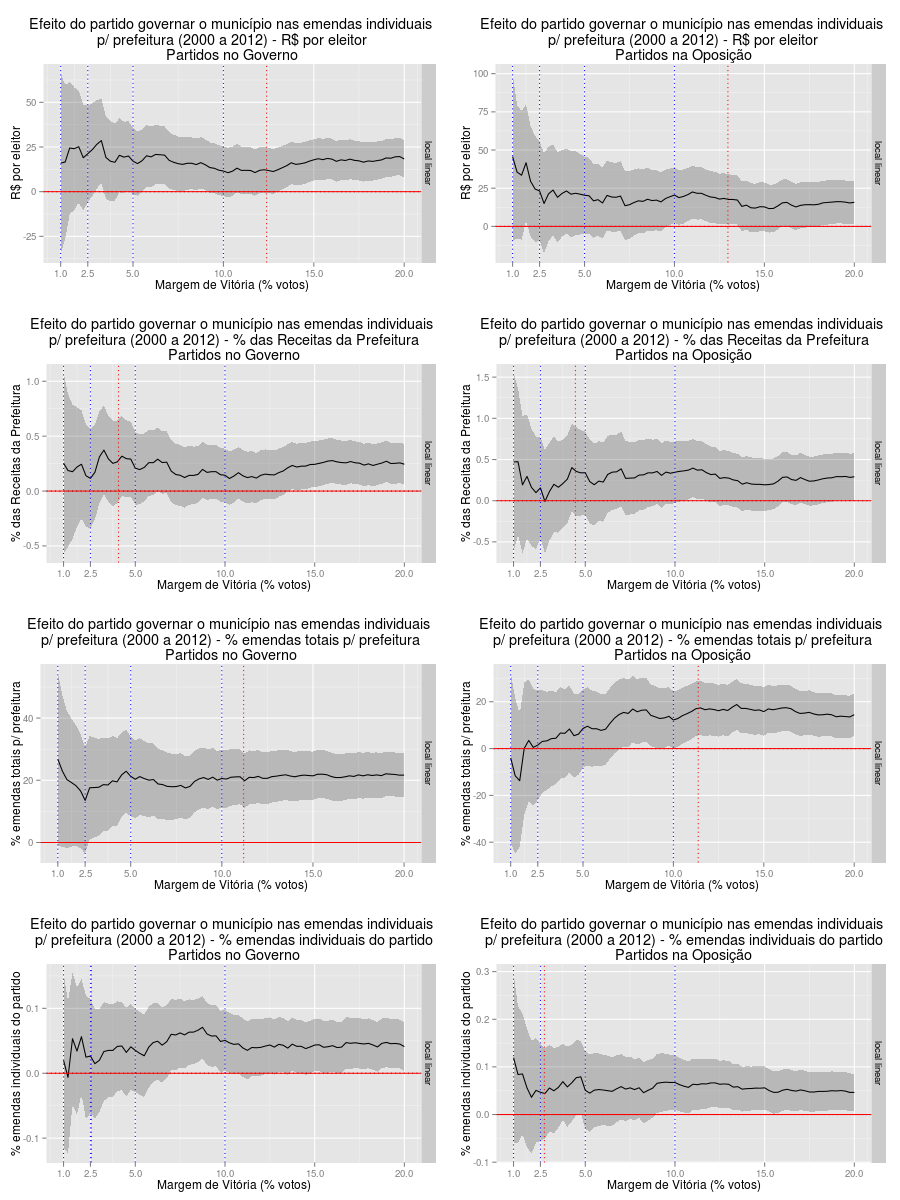
\includegraphics[scale=0.50]{c2g13.png}
	\caption{Efeito do Tratamento nas emendas individuais apresentadas por parlamentares do partido nos três últimos anos do mandato de prefeito por margem de vitória e separado por partidos no governo e partidos na oposição (2004 a 2012).}
	\label{fig:c2g13}
\end{figure}

A redução do número de observações para os dois cojuntos de dados -- parlamentares do governo e da oposição -- tem como efeito a perda de significância estatística em quase todas as medidas. Vale notar que há mais partidos no grupo de governistas do que no grupo oposicionistas. Assim, mesmo havendo um grande número de observações para DEM e PSDB, o grupo formado por estes dois partidos conta com menos observações do que o outro grupo.

De maneira geral, os gráficos para cada um desses dois conjuntos são bastante semelhantes entre si. Há duas diferenças a se notar. Praticamente não há efeito do tratamento para partidos da oposição. Este resultado, porém, pode ser consequência do número mais baixo de observações e não seria prudente afirmar exclusivamente a partir deste critério que partidos no governo ou na oposição têm diferenças entre si.

A segunda diferença reside nos gráficos para os dois grupos em que $Y_{i}^{pref}$ é medido como total de emendas de um partido para um município sobre a soma das emendas de todos os partidos para o mesmo município. Esta é a única situação em que há diferenças relevantes entre governistas e oposicionistas, pois o efeito é bastante claro para o primeiro e inexistente para o segundo grupo. Novamente, porém, este dado é insuficiente para apontar que há diferenças reais entre os parlamentares de cada um dos grupos. A inclusão dos casos em que $Y_{i}^{pref}=0$, cujos gráficos são apresentados no Anexo, torna as diferenças entre os grupos ainda menos claras.

Seria possível neste capítulo repetir a análise dos efeitos heterogêneos apresentados no Capítulo~\ref{cap:eleicoes}. Por exemplo, o efeito estimado para municípios menores, mais pobres ou mais dependentes de diferenças poderia ser maior do que o efeito estimado para municípios maiores, mais ricos ou menos dependentes dos demais níveis de governo. Entretanto, os resultados separados por características municipais não apontam para efeitos heterogêneos relevantes. Tal como aconteceu com a separação por posição em relação ao governo, a divisão dos dados em subconjuntos de características municipais não revela diferenças importantes. Os gráficos do efeito estimado por característica municipal constam do Anexo.

\begin{figure}[htp]
	\centering
	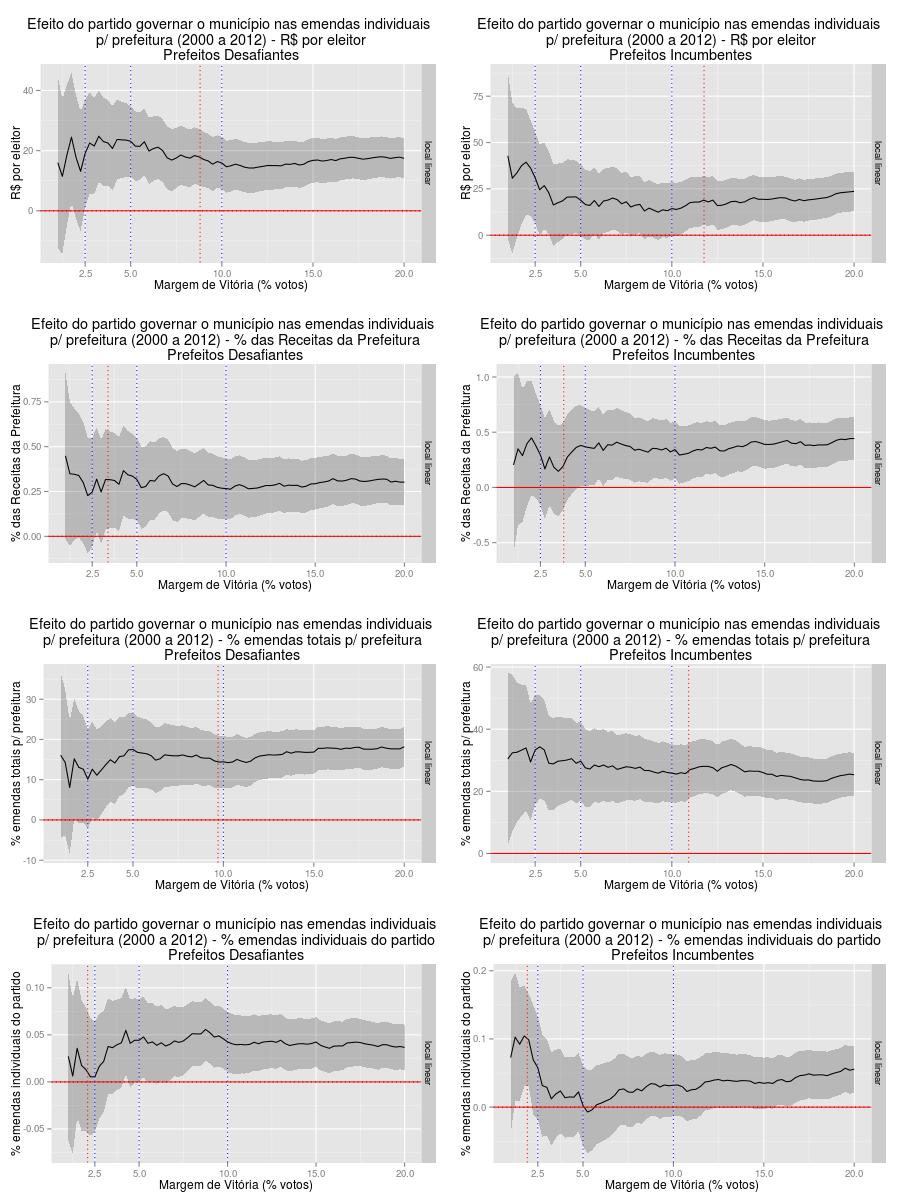
\includegraphics[scale=0.50]{c2g14.png}
		\caption{Efeito do Tratamento nas emendas individuais apresentadas por parlamentares do partido nos três últimos anos do mandato de prefeito por margem de vitória e separado por contexto eleitoral local (2000 a 2012).}
	\label{fig:c2g14}
\end{figure}

Finalmente, no primeiro capítulo pudemos verificar que há diferenças notáveis para os casos em que o partido já governava o município em relação aos casos em que o partido ainda não governava. A Figura~\ref{fig:c2g14} apresenta os resultados para as quatro medidas de $Y_{i}^{pref}$ para cada uma das situações. A diferença central é que os valores estimados para as quatro medidas nos casos em que o partido já governava o município anteriormente são em geral maiores, ou seja, esperamos um efeito nas situações em que partido se mantém no governo municipal. Os intervalos de confiança do efeito estimado são bastante grandes e nem sempre podemos dizer que $\rho$ é diferente de zero, ainda que em todos os gráficos da Figura~\ref{fig:c2g14} haja pelo menos um ponto para margens abaixo 5\% em que o efeito é estatisticamente diferente de zero.

Vamos agora analisar os efeitos do partido governar o municío nas emendas individuais cujos beneficiários são as Entidades Sem Fins Lucrativos localizadas em determinado município e não mais as prefeituras.

\subsection{Emendas individuais ao Orçamento e Entidades Sem Fins Lucrativos: hipóteses}

Com certa frequência vemos notícias sobre escândalos envolvendo transferências de recursos do governo federal e dos governos estaduais a Entidades Sem Fins Lucrativos. A existência de controles burocráticos menores seriam responsáveis pela opção de políticos no Legislativo e no Executivo enviar recursos para apoiadores políticos ou mesmo desviar recursos públicos. Entretanto, sabe-se muito pouco sobre a relação entre o Estado e organizações da sociedade civil que recebem recursos estatais para a produção de fins públicos. As ESFLs formam um conjunto bastante grande e diverso de organizações e não é uma única forma de relação entre entidades que fazem parte deste conjunto e o Estado (para discussões e dados sobre o tema ver \citealp*{Lopez2012} e \citealp*{Lopez2013})

O objetivo nesta seção é examinar se o fato do partido governar o município ou não influencia nas decisões dos parlamentares em enviarem recursos a ESFLs localizadas no município. Mas qual é a relação entre a filiação do prefeito e decisão dos parlamentares em relação a organizações não formalmente vinculadas com a prefeitura?

A suspeita central é que ESFLs podem configurar um caminho alternativo para parlamentares obterem apoio de lideranças locais em municípios que lhes interessam eleitoralmente, mas que são governados por partidos opostos ao seu. Este cenário seria particularmente importante se, por exemplo, um deputado foi eleito com votos em um município governado por um aliado e, na metade de seu mandato parlamentar, esta localidade passou a ser governado por outro partido. O município continua sendo eleitoralmente atrativo para o deputado que, neste novo cenário, não pode mais contar com o apoio do chefe do Executivo local.  

Ainda que o prefeito seja uma liderança política de destaque no município, certamente concorre com atores locais além dos membros do Legislativo. Pessoas à frente de organizações comunitárias, igrejas, sindicatos, movimentos sociais, organizações filantrópicas -- apenas para listar algumas -- podem ocupar o importante papel de intermediar a relação dos cidadãos e eleitores com seus representantes nos demais níveis de governo. Se os prefeitos são um caminho interno ao partido para se chegar aos eleitores, essas lideranças podem representar um caminho externo.

Infelizmente, não é possível atribuir a lideranças locais um partido e testar se a vinculação com os deputados federais explica as transferências às suas organizações, como no caso de prefeitos. Ainda assim, é viável observar se o conjunto de organizações no município tendem a receber mais recursos de um partido quando este perde as eleições para prefeito, sendo esta a principal hipótese a ser testada na próxima subseção. Examinando transferências federais a ESFLs -- e não apenas as emendas parlamentares que beneficiam ESFLs -- \citet{Bueno2014} aponta que o Governo Federal adota como estratégia o envio de recursos para tais organizações em municípios governados por oposicionistas.

O principal problema de testar a hipótese de ESFLs como alternativa à prefeitura para obtenção de apoio político local é que prefeitos podem também ter interesse que outras organizações no município, além da prefeitura, recebam recursos oriundos de outros níveis de governo. Em primeiro lugar, ESFLs estão sujeitas a menos controles burocráticos para executar recursos federais e estaduais do que as prefeituras. Neste caso, a ESFL é uma alternativa à prefeitura adotada pelo próprio governante local, e não por um parlamentar que tem interesse no município mas não tem a cooperação da prefeitura. Em segundo, prefeitos talvez contem com o apoio político das entidades no município. Obter recursos com deputados federais para tais organizações pode ser um objetivo estratégico do prefeito para a obtenção de apoio local. Se essas conjecturas forem verdadeiras, devemos esperar uma relação positiva entre o partido vencer as eleições municipais e os parlamentares do partido enviarem destinarem recursos a ESFLs do município.

É possível também que as duas hipóteses sejam verdadeiras e que os mecanismos por trás de uma e de outra coexistam. Neste caso, um conjunto de organizações no município serviria de rota alternativa para obter apoio local para parlamentares de partidos de oposição ao partido do prefeito e outro conjunto seria formado por organizações que recebem recursos justamente pela ação do governante local. Infelizmente, é impossível separar esses dois conjuntos de organizações locais e esta restrição deve ser levada em consideração na análise dos resultados a seguir.

\subsection{Emendas individuais ao Orçamento e Entidades Sem Fins Lucrativos: resultados}

A Figura \ref{fig:c2g15} apresenta os resultados para as quatro medidas de $Y_{i}^{esfl}$, sendo elas o total de emendas apresentas pelos parlamentares do partido que beneficiam ESFLs no município: 1- por eleitor; 2- como proporção das receitas da prefeitura; 3- como proporção do total destinados a ESFLs do município por parlamentares de quaisquer partidos; e 4- como proporção do total de recursos destinados por parlamentares do partido a todas as ESFLs do país. Ainda que no segundo caso o denominador seja um atributo da prefeitura (receitas totais), e não do conjunto de ESFLs no município, a variável medida desta forma nos permite comparar o volume de recursos destinado a ESFLs com o quanto o Executivo local tem à disposição para produzir políticas locais, contratar pessoal, etc. Tal como se procedeu até o momento, estão incluidas apenas observações em que $Y_{i}^{esfl}>0$ e os gráficos para $Y_{i}^{esfl} \geq 0$ são apresentados no Anexo.

\begin{figure}[htp]
	\centering
	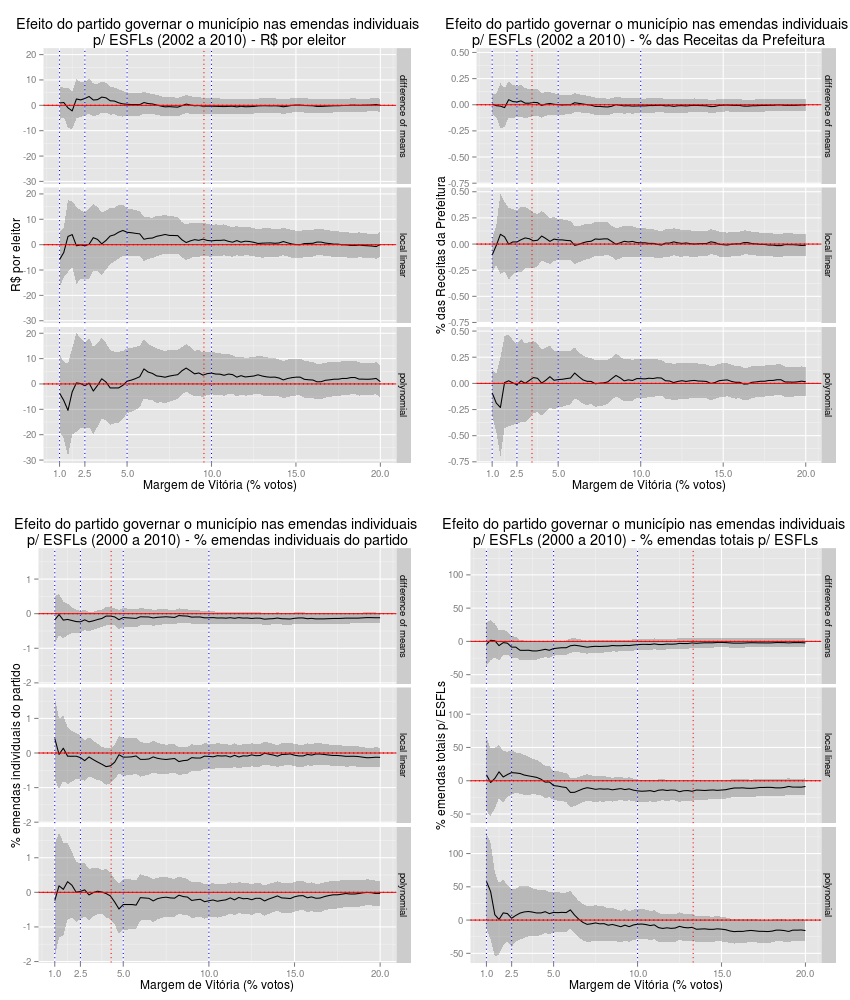
\includegraphics[scale=0.50]{c2g15.png}
		\caption{Efeito do Tratamento nas emendas individuais apresentadas por parlamentares do partido beneficiam Entidades Sem Fins Lucrativos nos três últimos anos do mandato de prefeito por margem de vitória (2000 a 2012).}
	\label{fig:c2g15}
\end{figure}

Todos os resultados apontam para uma única direção: não há evidências de que o partido no governo municipal não impacta na decisão dos parlamentares apresentarem emendas para ESFLs do município. Para as duas últimas medidas de $Y_{i}^{esfl}$ e para $\rho$ estimado por diferença de médias, há algum indicativo de que o tratamento tem efeito negativo, ou seja, de que parlamentares enviam mais recursos a ESFLs em municípios não governados pelo próprio partido do que para os demais. Além disso, quando da inclusão dos casos em que $Y_{i}^{esfl} \geq 0$ (apresentados no Anexo), é possível encontrar alguma evidência de que $\rho$ é menor e estatisticamente diferente de zero. Sob os critérios adotados nesta pesquisa, porém, é mais prudente afirmar que não há impacto do resultado nas eleições municipais sobre a decisão do deputados federais em relação a ESFLs.

Existem pelo menos três explicações possíveis para o resultado nulo. A primeira é que de fato não há relação entre o partido no governo municipal e a decisão dos partidos no Congresso. Entretanto, o resultado nulo pode ser também consequência de um número muito baixo de observações com $Y_{i}^{esfl}>0$ e, consequentemente, da existência de poucas eleições municipais decididas por uma margem pequena de votos. A existência de poucas observações disponíveis para a análise é também a razão pela qual não convém proceder o exame de efeitos heterogêneos do tratamento, procedimento adotado para a análise das emendas parlamentares que beneficiam prefeituras.

Por fim, o resultado nulo pode ser reflexo da não separação dos dois conjuntos de organizações na totalidade de EFSLs de um município entre aquelas aliadas ao prefeito -- e para as quais o mandatário local tentará obter recursos -- e as entidades que poderiam servir como alternativa para obtenção de apoio político local para parlamentares em oposição ao prefeito. Se os sinais para cada conjunto de organizações é oposto, tratá-los de forma indiferenciada interfere na estimação de $\rho$.

\section{Conclusão: \emph{conexão partidária}, prefeitos e deputados federais}

O propósito central do capítulo foi examinar se deputados federais apresentam emendas individuais que beneficiam prioritariamente prefeituras governadas pelo seu partido. O argumento principal é que os reais demandantes de \emph{pork} são lideranças locais capazes de influenciar os resultados eleitorais futuros de um parlamentar e que as emendas apresentadas por deputados federais revelam os vínculos partidários entre legisladores e governantes locais. Nos termos da literatura rapidamente debatida no início do capítulo, a conexão que explica as decisões parlamentares é \emph{partidária} e não necessariamente \emph{eleitoral}.

As evidências encontradas no capítulo dão suporte a este argumento. Podemos observar impactos relevantes do partido governar o município sobre a decisão alocativa dos deputados fedearis para diferentes maneiras de medir o total de emendas individuais que beneficiam governos locais.

A investigação se extendeu também às emendas individuais que beneficiam ESFLs. Buscou-se evidências de que estas organizações apresentariam uma alternativa para a obtenção político em municípios governados por prefeitos opositores a um parlamentar. Os resultados encontrados no exame desta hipótese são nulos e não é possível distinguir a ausência de efeitos da qualidade do teste realizado.

Em conjunto com as conclusões tentativas do primeiro capítulo, a avaliação do resultados até este momento na tese tornam crível a narrativa apresentada. Prefeitos são, de um lado, atores políticos fundamentais para a construção de candidaturas vitoriosas nas eleições proporcionais e atuam em prol de membros de seu partido. A cooperação e articulação entre membros de uma organização partidária é um elemento central da competição eleitoral. Por outro lado, prefeitos são os demandantes de benefícios geograficamente localizados. A coordenação entre parlamentares e governantes locais influencia os resultados das decisões no Congresso Nacional.

Tal como no capítulo anterior, ainda há alguns aspectos da análise que podem e devem ser melhorados na pesquisa apresentada nesta etapa. Em primeiro lugar, com esforços mais amplos de coleta de dados é possível reatroagir a análise para as eleições de 1996 e incluir as eleições de 2012. Particularmente no caso das organizações não estatais beneficiadas, é necessário ampliar o número de observações para diferenciar a ausência de resultados pela qualidade da estimativa da ausência de resultados pela inexstência de efeitos. Também seria importante testar se os resultados se mantém ao substituir os valores apresentados das emendas individuais pelos valores efetivamente transferidos às prefeituras e ESFLs. Ainda que os valores apresentados capturem com mais fidelidade o que se pretende medir, alterações na variável podem contribuir para a validação dos resultados e para a melhor compreensão do fenômeno. Por fim, incluir os efeitos da migração partidária de prefeitos na análise deve ser um objetivo futuro.